\documentclass{beamer}
\usetheme{Antibes}
\usecolortheme{beaver}

\usepackage[english]{babel}
\usepackage{lmodern}
\usepackage[T1]{fontenc}
\usepackage[utf8]{inputenc}
\usepackage{amsmath}
\usepackage{amssymb}
\usepackage{amsfonts}
\usepackage{bm}
\usepackage{graphicx}
\usepackage{subcaption}
\usepackage{mathtools}
\usepackage{color}
\usepackage{booktabs}
\usepackage{tikz}


\newcommand{\bx}{\bm{x}}
\newcommand{\by}{\bm{y}}
\newcommand{\bu}{\bm{u}}
\newcommand{\btheta}{\bm{\theta}}

\newcommand{\trans}{f}
\newcommand{\obs}{g}
\newcommand{\sprior}{p}
\newcommand{\pprior}{\pi}
\newcommand{\prop}{q}
\newcommand{\dx}[1]{\mathrm{d}{#1}}


\begin{document}
    \author{%
        Bc. Tom\'a\v{s} Kala \\
        Supervisor: Ing. Kamil Dedecius, PhD.}
    \title{Bayesian Parameter Estimation of State-Space Models with Intractable Likelihood}
    %\subtitle{}
    %\logo{}
    %\institute{}
    \date{June 20, 2019}
    %\subject{}
    %\setbeamercovered{transparent}
    %\setbeamertemplate{navigation symbols}{}
    \begin{frame}[plain]
    \maketitle
    \end{frame}

    
    \begin{frame}
    \frametitle{State-Space Model (SSM)}
    
    \begin{columns}
        \begin{column}{0.5\textwidth}
            \begin{figure}[ht]
                \centering
                \resizebox{\columnwidth}{!}{%
                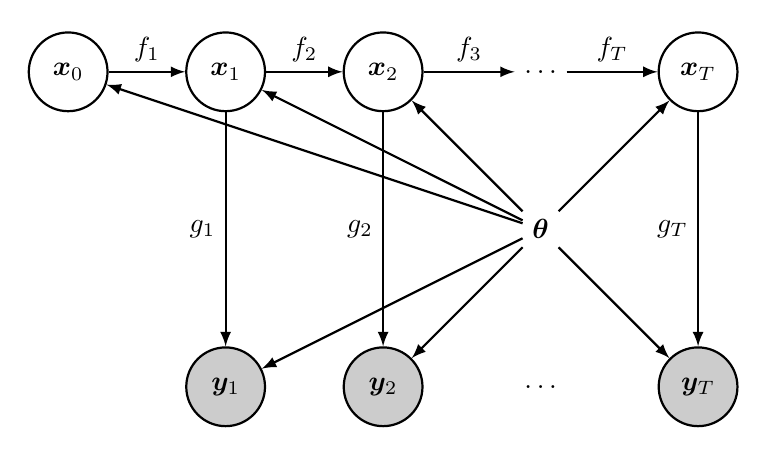
\begin{tikzpicture}
                % Style
                \tikzstyle{main}=[circle, minimum size = 10mm, thick, draw =black!80, node distance = 16mm]
                \tikzstyle{connect}=[-latex, thick]
                
                % Nodes X
                \node[main,shape=circle,draw=black](X0) at (1,4) {$\bx_0$};
                \node[main,shape=circle,draw=black](X1) at (3,4) {$\bx_1$};
                \node[main,shape=circle,draw=black](X2) at (5,4) {$\bx_2$};
                \node[](Xdots) at (7,4) {$\ldots$};
                \node[main,shape=circle,draw=black](XT) at (9,4) {$\bx_T$};
                
                % Node theta
                \node[](theta) at (7,2) {$\btheta$};
                
                % Nodes Y
                \node[main,shape=circle,draw=black,fill=black!20](Y1) at (3,0) {$\by_1$};
                \node[main,shape=circle,draw=black,fill=black!20](Y2) at (5,0) {$\by_2$};
                \node[](Ydots) at (7,0) {$\ldots$};
                \node[main,shape=circle,draw=black,fill=black!20](YT) at (9,0) {$\by_T$};
                
                % Edges XX
                \path [->] (X0) edge[connect] node[left] [above] {$\trans_1$} (X1);
                \path [->] (X1) edge[connect] node[left] [above] {$\trans_2$} (X2);
                \path [->] (X2) edge[connect] node[left] [above] {$\trans_3$} (Xdots);
                \path [->] (Xdots) edge[connect] node[left] [above] {$\trans_T$} (XT);
                
                % Edges XY
                \path [->] (X1) edge[connect] node[left] [left] {$\obs_1$} (Y1);
                \path [->] (X2) edge[connect] node[left] [left] {$\obs_2$} (Y2);
                \path [->] (XT) edge[connect] node[left] [left] {$\obs_T$} (YT);
                
                % Edges theta X
                \path [->] (theta) edge[connect] node[left] {} (X0);
                \path [->] (theta) edge[connect] node[left] {} (X1);
                \path [->] (theta) edge[connect] node[left] {} (X2);
                \path [->] (theta) edge[connect] node[left] {} (XT);
                
                % Edges theta Y
                \path [->] (theta) edge[connect] node[left] {} (Y1);
                \path [->] (theta) edge[connect] node[left] {} (Y2);
                \path [->] (theta) edge[connect] node[left] {} (YT);
                \end{tikzpicture}
                }
                \label{fig:graphical-model}
            \end{figure}            
        \end{column}
%
        \begin{column}{0.5\textwidth}
            \begin{equation*}
            \begin{split}
            \bx_0 \mid \btheta & \sim \sprior(\bx_0 \mid \btheta), \\
            \bx_t \mid \bx_{t-1}, \btheta & \sim \trans_t(\bx_t \mid \bx_{t-1}, \btheta), \\
            \by_t \mid \bx_t, \btheta & \sim \obs_t(\by_t \mid \bx_t, \btheta), \\
            \btheta & \sim \pprior(\btheta).
            \end{split}
            \end{equation*}
        \end{column}
    \end{columns} 

    \begin{itemize}
        \item The posterior of $\btheta$ takes the form of
        \begin{equation*}
        p(\btheta \mid \by_{1:T}) \propto p(\by_{1:T} \mid \btheta) \pprior(\btheta),
        \end{equation*}
        where
        \begin{equation*}
         p(\by_{1:T} \mid \btheta) = \int p(\bx_{0:T}, \by_{1:T} \mid \btheta) \; \dx{\bx_{0:T}}.
        \end{equation*}
    \end{itemize}
    \end{frame}

    \begin{frame}
    \frametitle{Particle filter}
    \begin{itemize}
        \item Use weighted particles $\left\{\left(\bx_t^{(i)}, w_t^{(i)}\right) : i = 1, \ldots, N\right\}$ to approximate the filtering distribution $p(\bx_t \mid \by_{1:t}, \btheta)$.
        \item Simulate the particles $\bx_t^{(i)} \sim \trans_t(\bx_t \mid \bx_{t-1}^{(i)})$ and weight them according to $w_t^{(i)} = \obs_t(\bx_t^{(i)} \mid \by_t, \btheta)$.
        \item An unbiased likelihood estimator is
        \begin{equation*}
        \widehat{p}(\by_{1:T} \mid \btheta) = \prod_{t=1}^T \frac{1}{N} \sum_{i=1}^N w_t^{(i)}.
        \end{equation*}
        \item Problem: the observation model $\obs_t(\bx_t \mid \by_t, \btheta)$ must be known and probabilistic.
    \end{itemize}
    \end{frame}

    \begin{frame}
    \frametitle{Approximate Bayesian Computation (ABC)}
    \begin{columns}
        \begin{column}{0.45\textwidth}
            \begin{itemize}
                \item Use $\obs_t(\by_t \mid \bx_t, \btheta)$ to simulate pseudo-observations $\bu_t$.
                \item Determine $w_t^{(i)}$ based on the closeness of $\bu_t$ to the true $\by_t$ measured by a kernel function.
                \item A flexible and robust approach no longer requiring a probabilistic observation model.
            \end{itemize}
        \end{column}
%
        \begin{column}{0.5\textwidth}
            \begin{figure}
                \centering
                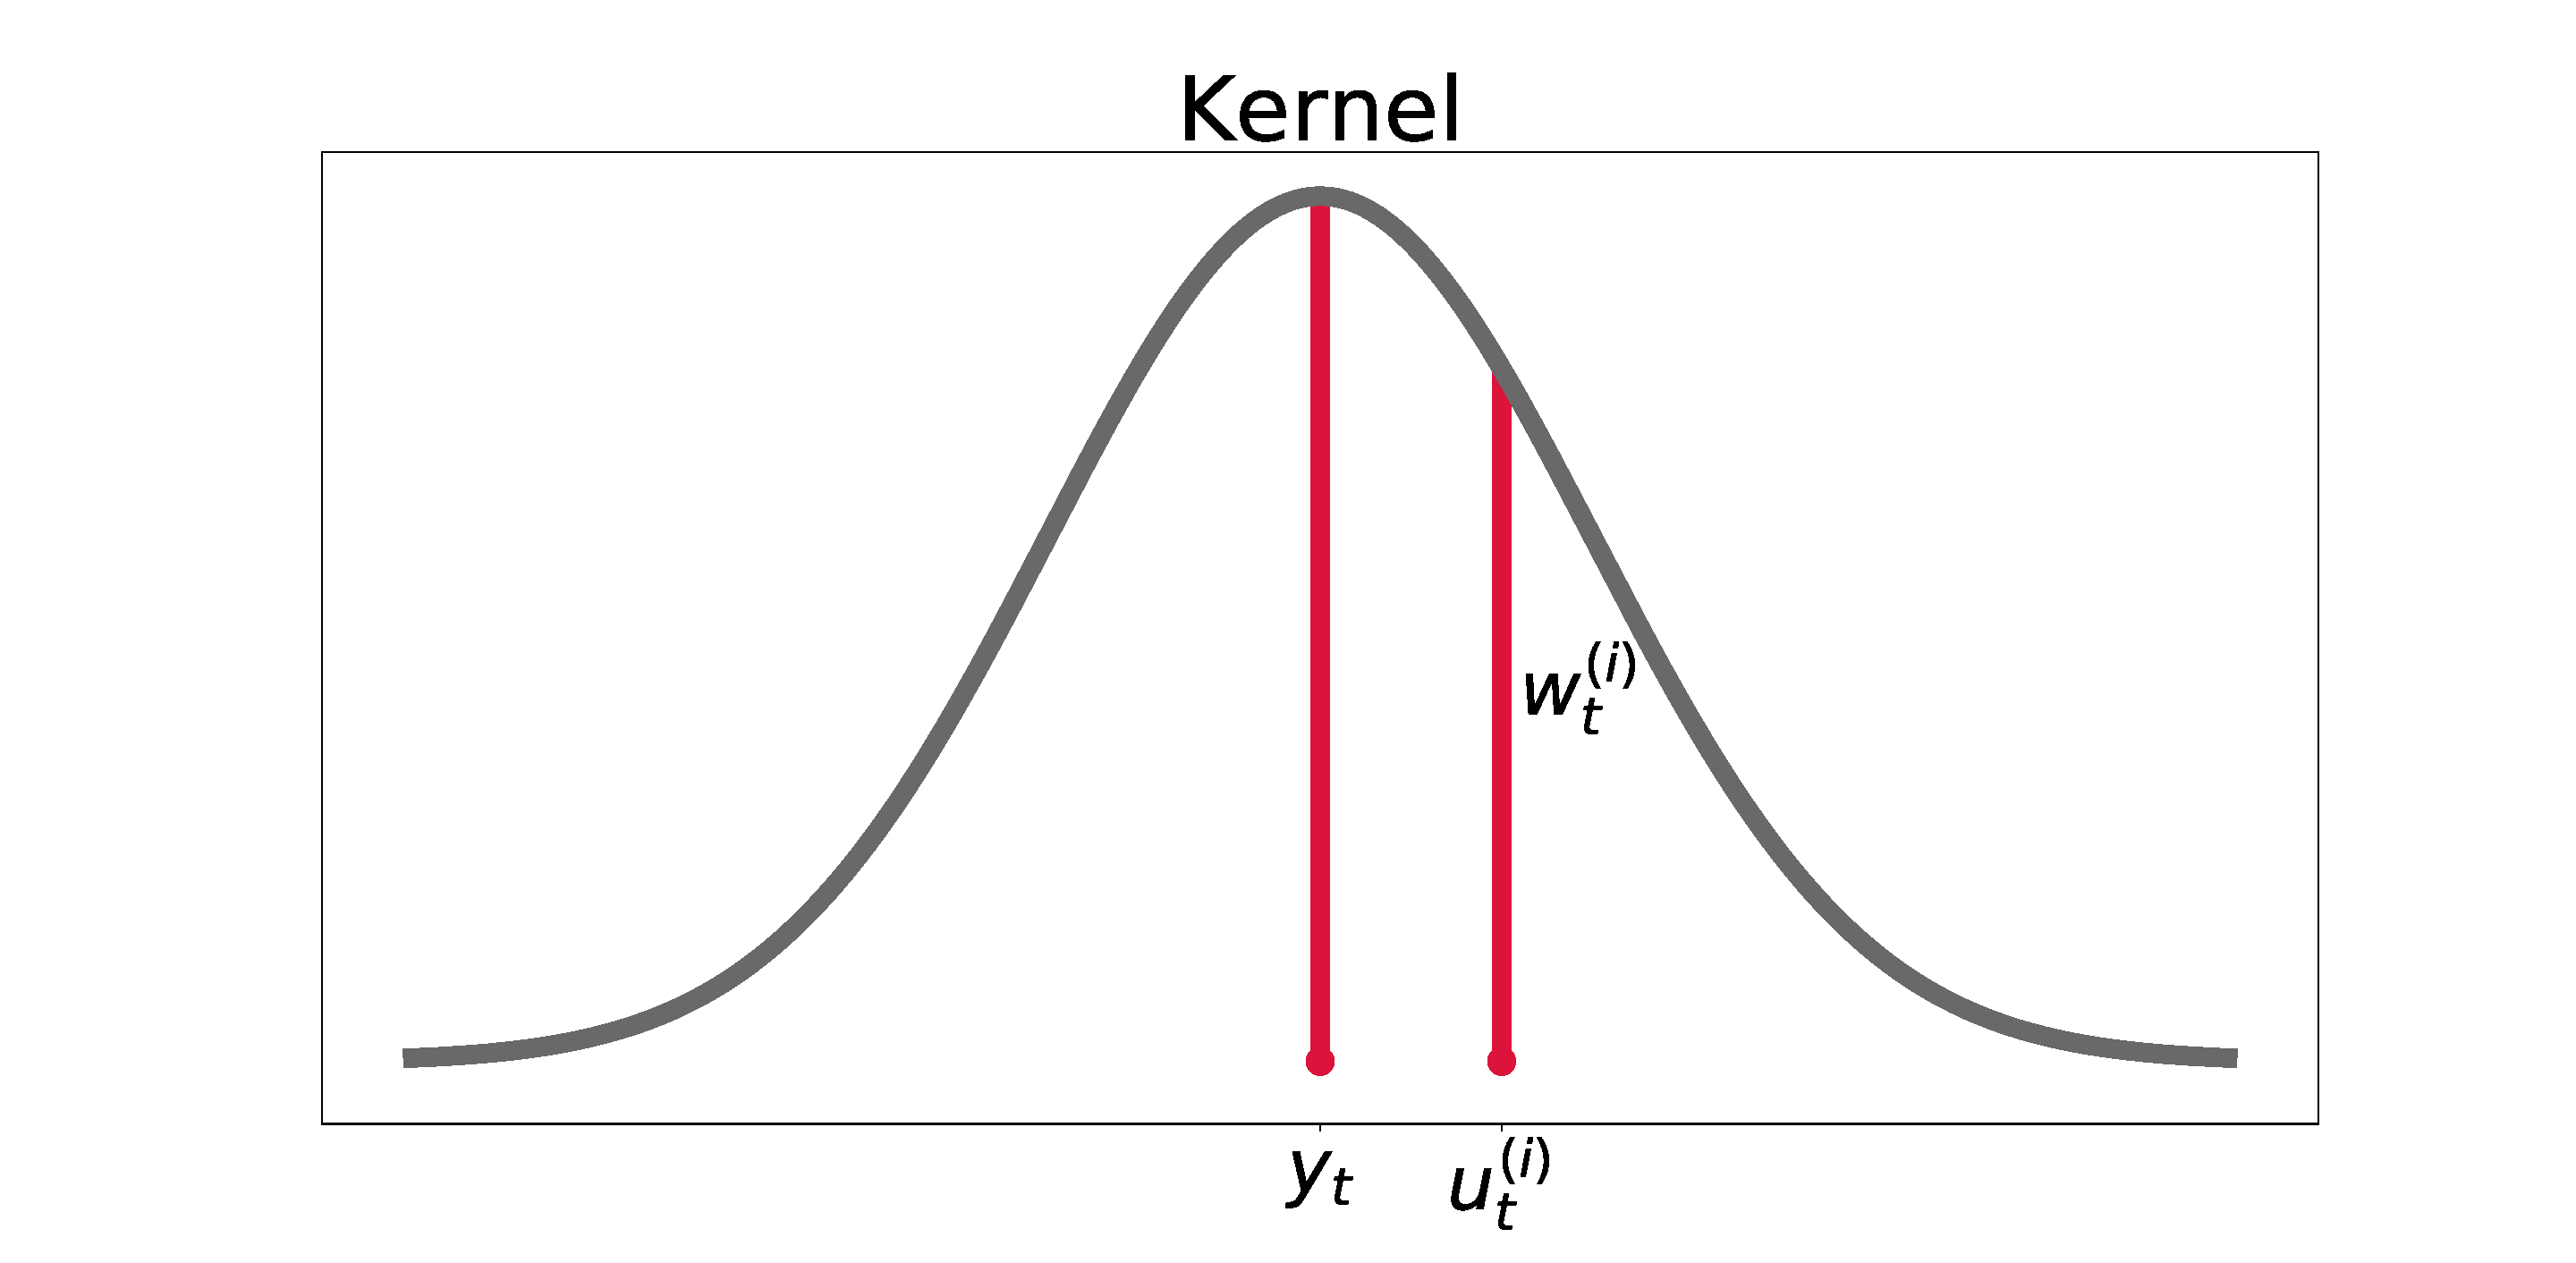
\includegraphics[width=\columnwidth]{images/kernel}
            \end{figure}
        \end{column}
    \end{columns}
    \end{frame}

    \begin{frame}
    \frametitle{Lotka-Volterra model}
    \begin{itemize}
        \item A simplified system of interacting prey ($\mathcal{X}_1$) and predator ($\mathcal{X}_2$) species described by
        \begin{equation*}
        \begin{split}
        \mathcal{R}_1 &: \quad \mathcal{X}_1 \to 2 \mathcal{X}_1, \\
        \mathcal{R}_2 &: \quad \mathcal{X}_1 + \mathcal{X}_2 \to 2 \mathcal{X}_2, \\
        \mathcal{R}_3 &: \quad \mathcal{X}_2 \to \emptyset. \\
        \end{split}
        \end{equation*}
        \item Assume $\by_t = \bx_t = \left(x_{1,t}, x_{2,t}\right)^\intercal$, Gaussian observation model and the unknown parameters to be $\btheta = \left(c_1, c_2, c_3\right)^\intercal$.
        \item Denoting the number of species $j$ present at the beginning of $\mathcal{R}_i$ by $p_{ij}$,
        \begin{equation*}
            c_i \prod_{j=1}^{2} \begin{pmatrix}
            x_{j,t} \\
            p_{ij}
            \end{pmatrix}
        \end{equation*} is the mean time to the next occurrence of $\mathcal{R}_i$ at time $t$.
    \end{itemize}
    \end{frame}

    \begin{frame}
    \frametitle{Lotka-Volterra model}
    \begin{columns}
        \begin{column}{0.45\textwidth}
            \begin{figure}
                \centering
                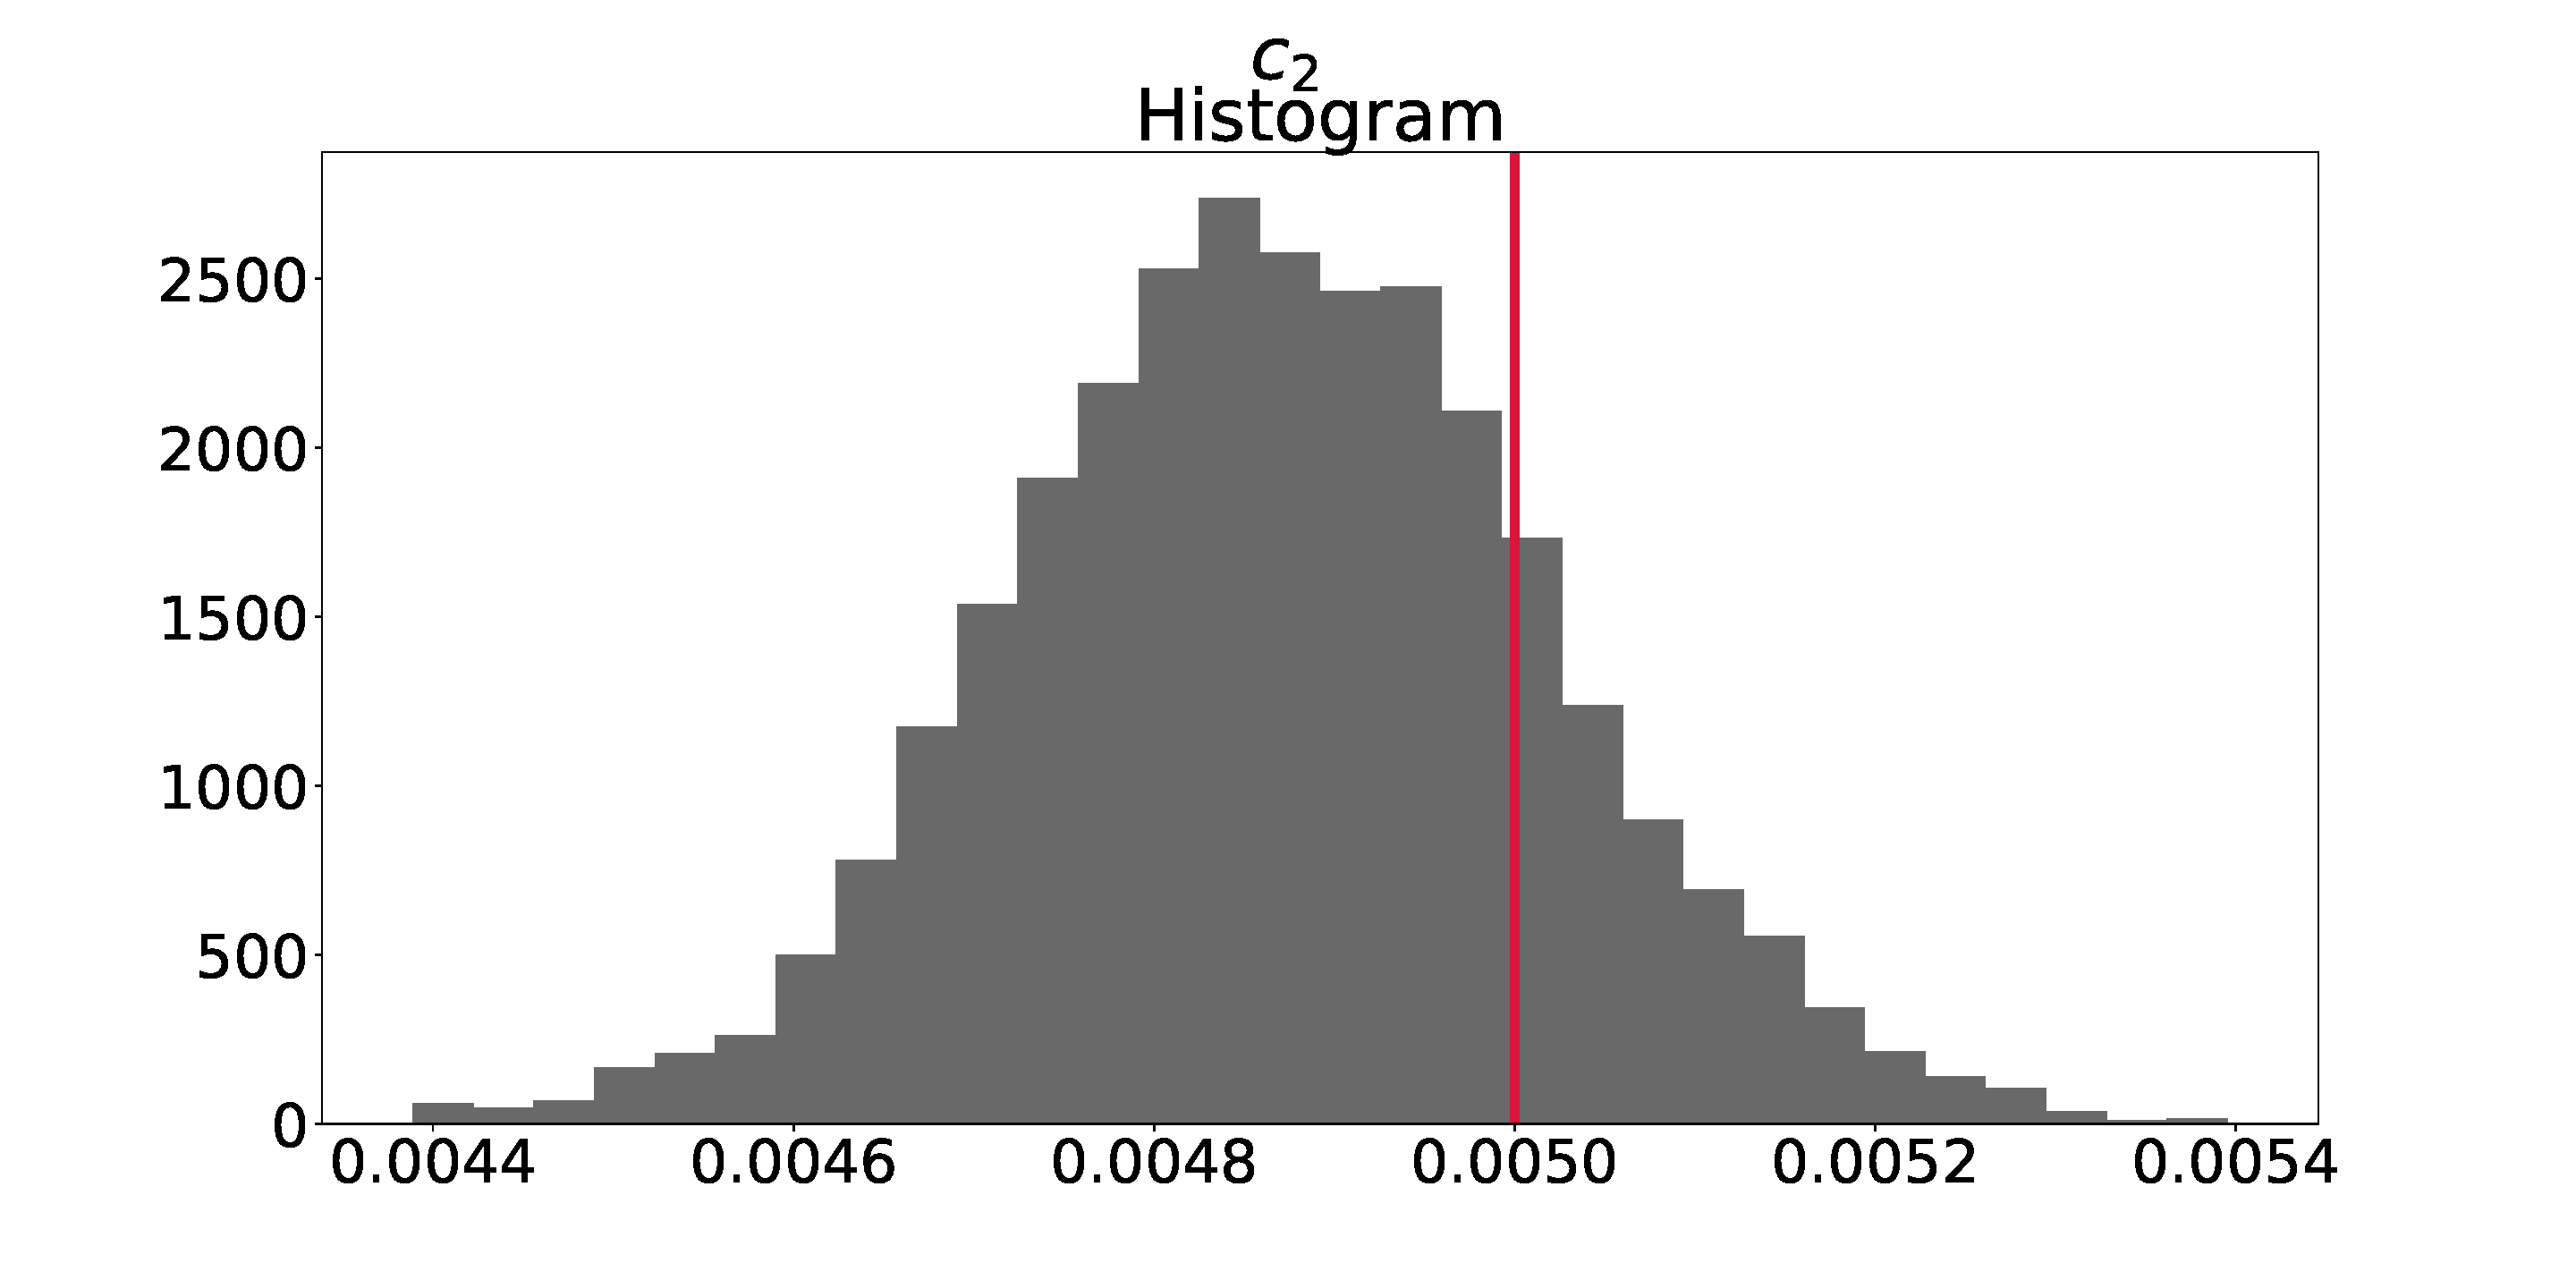
\includegraphics[width=\columnwidth]{images/lv_pf_g}
                \caption{Well-specified PF.}
            \end{figure}
        \end{column}
%
        \begin{column}{0.45\textwidth}
            \begin{figure}
                \centering
                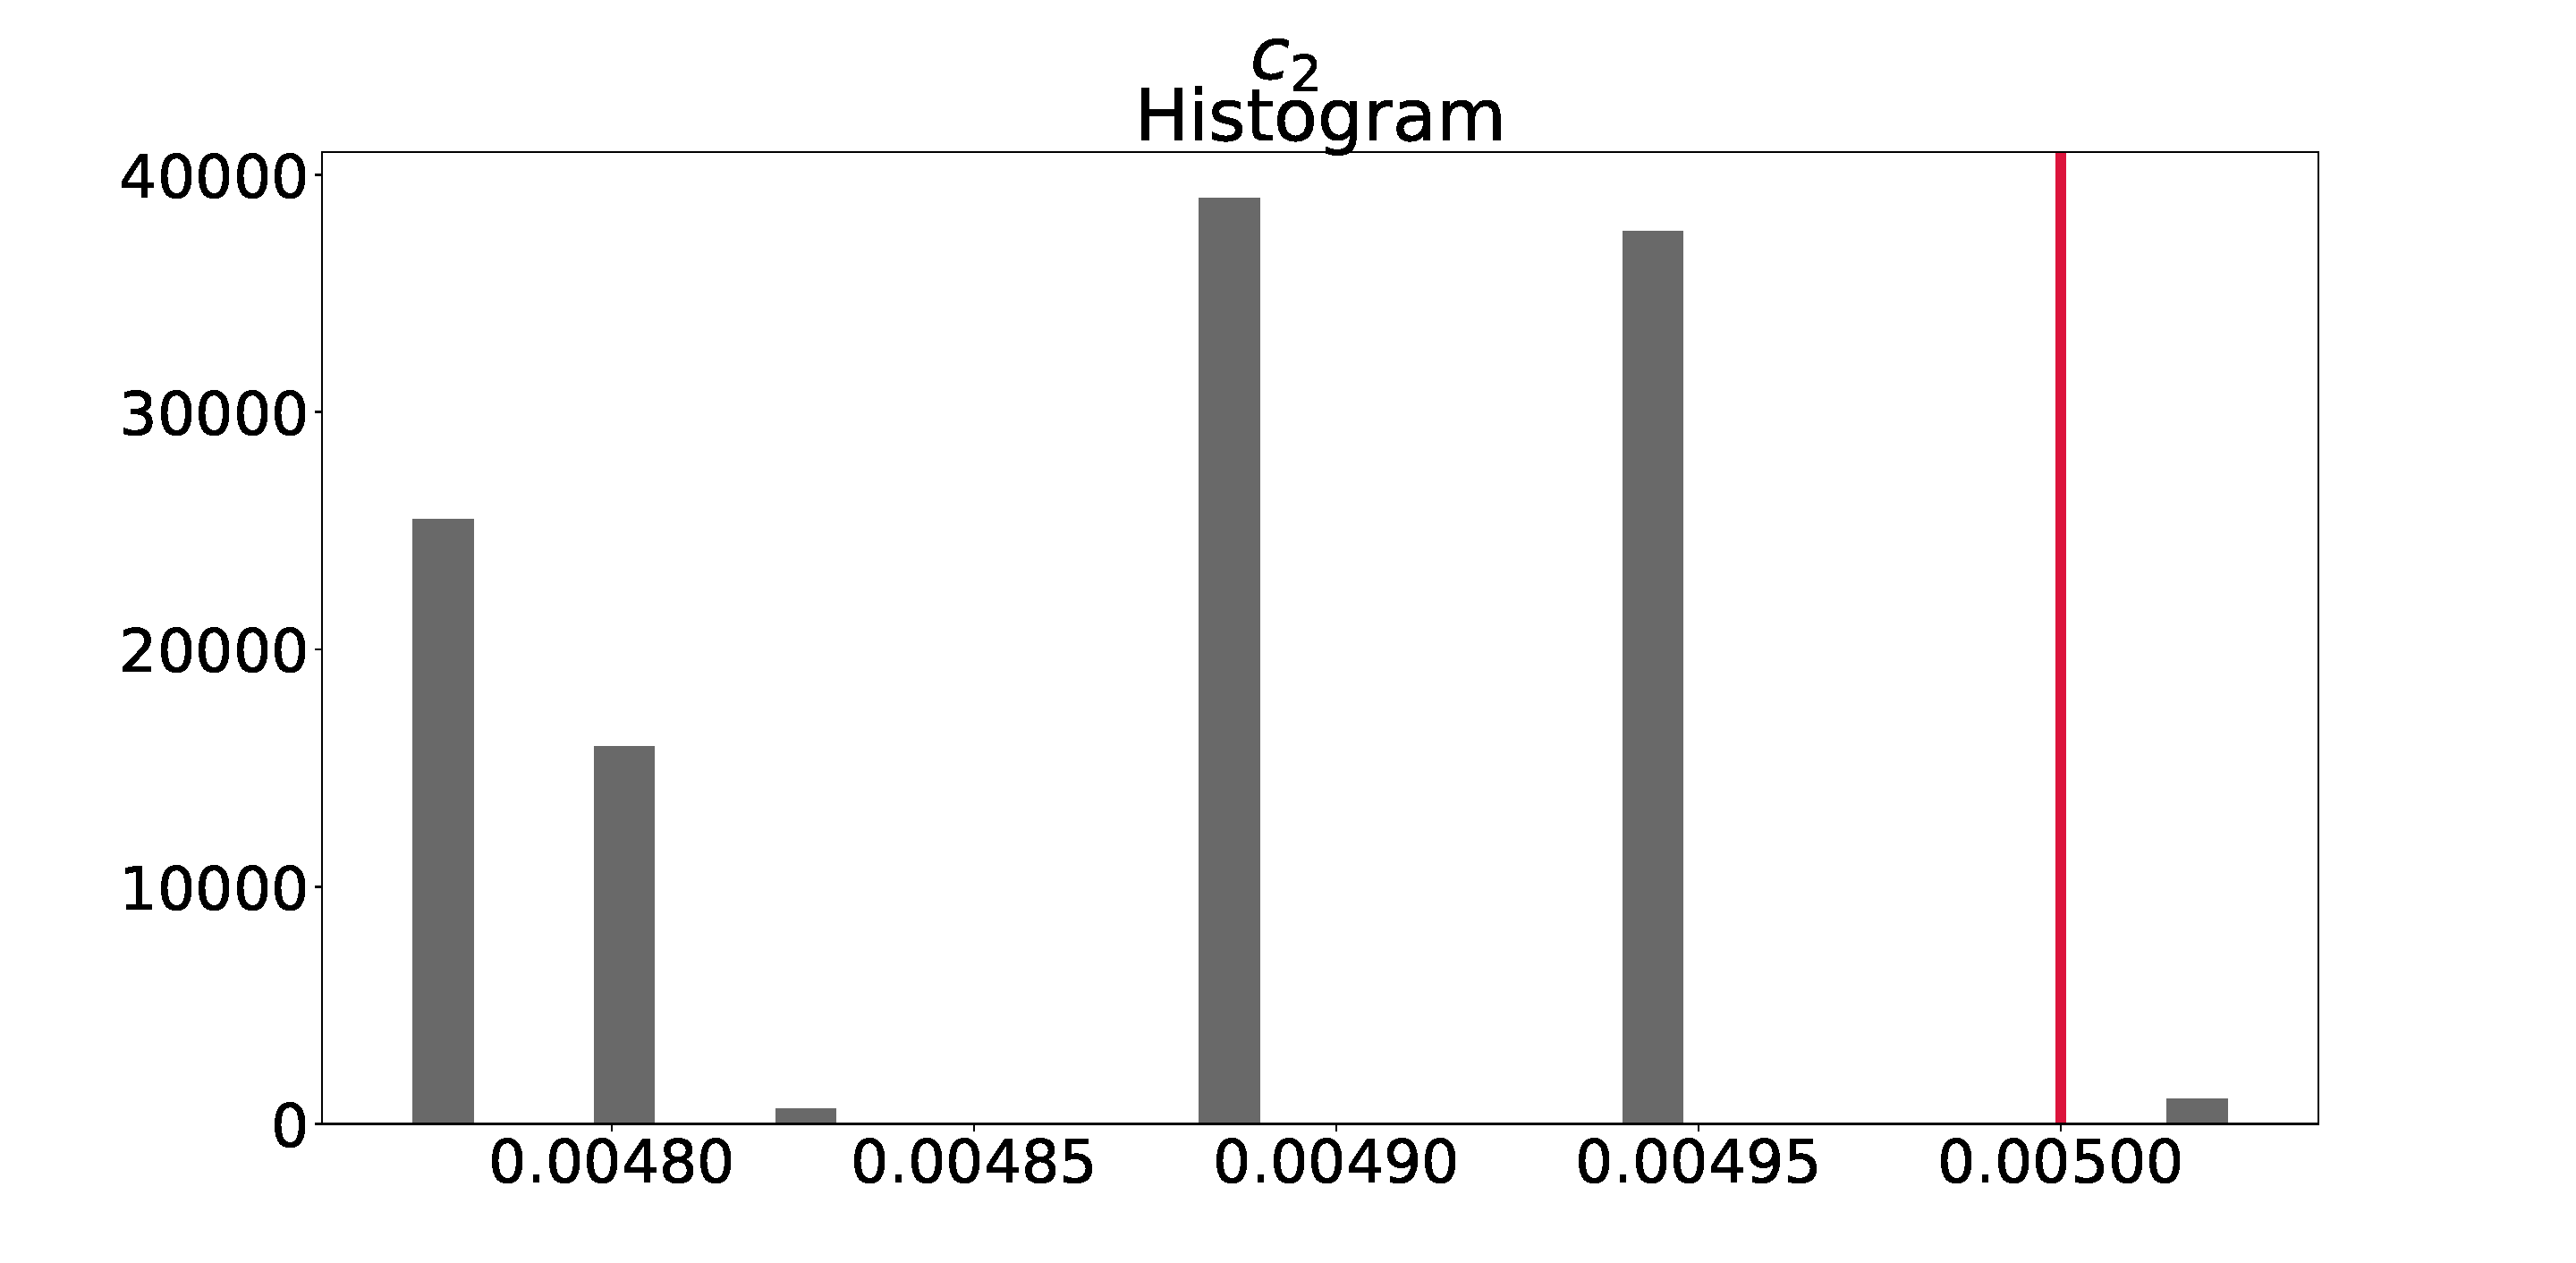
\includegraphics[width=\columnwidth]{images/lv_pf_c}
                \caption{Misspecified PF.}
            \end{figure}
        \end{column}
    \end{columns}

    \begin{columns}
        \begin{column}{0.45\textwidth}
            \begin{figure}
                \centering
                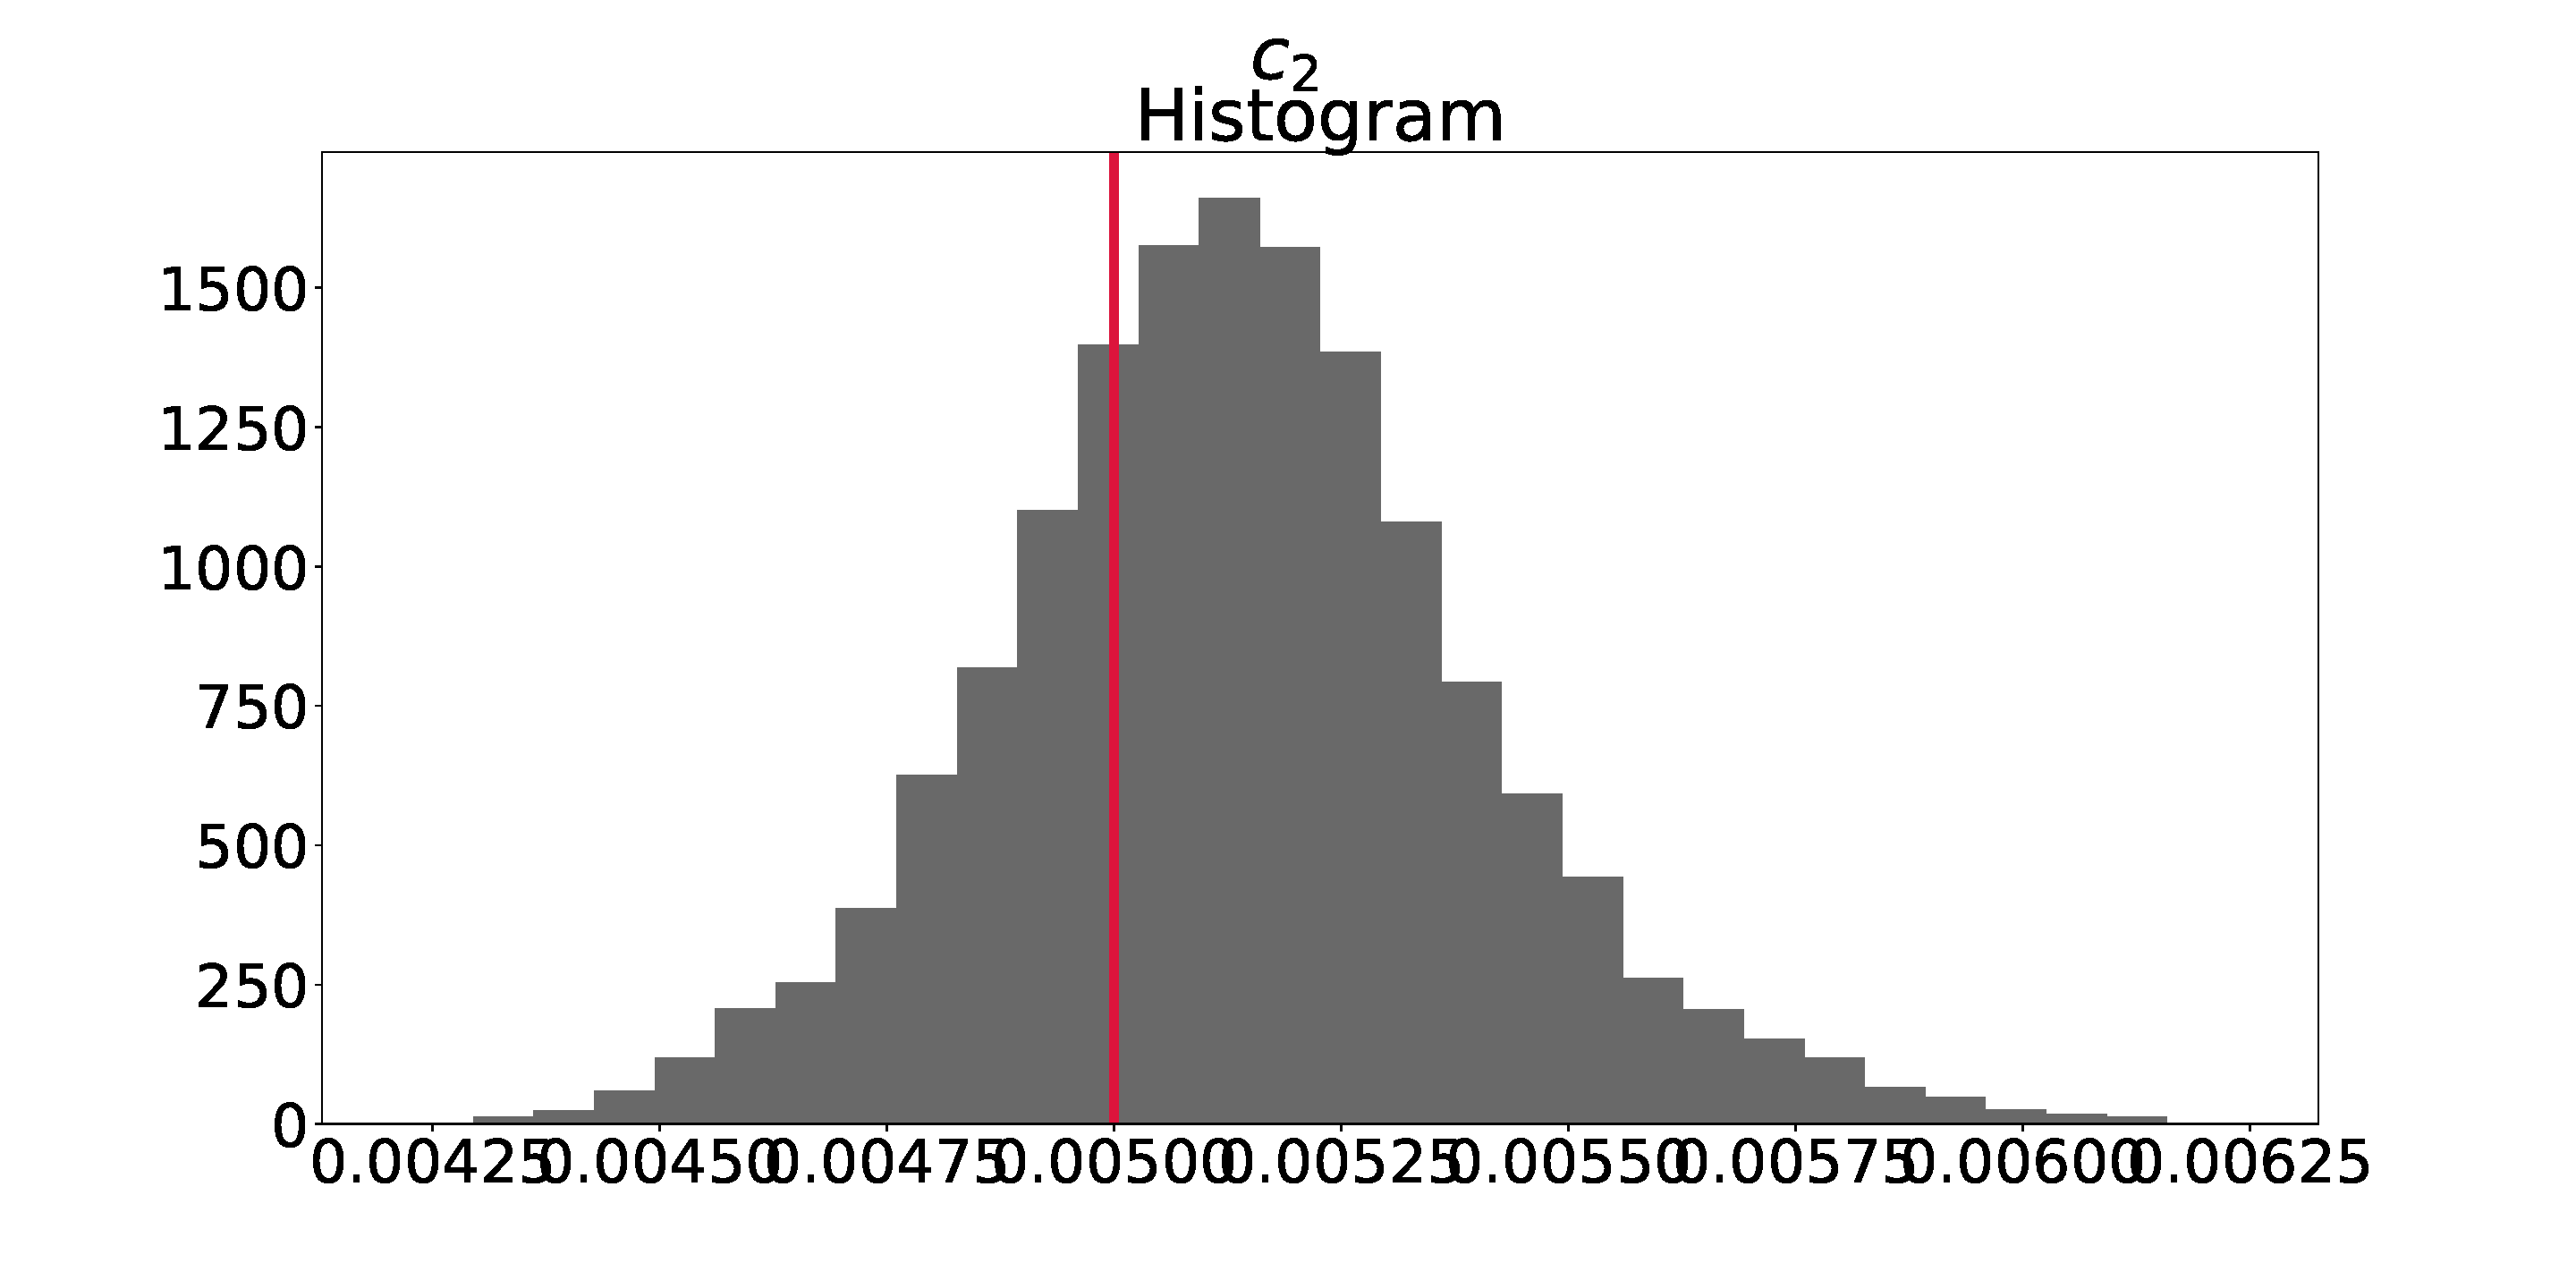
\includegraphics[width=\columnwidth]{images/lv_abc_g}
                \caption{Well-specified ABC.}
            \end{figure}
        \end{column}
        %
        \begin{column}{0.45\textwidth}
            \begin{figure}
                \centering
                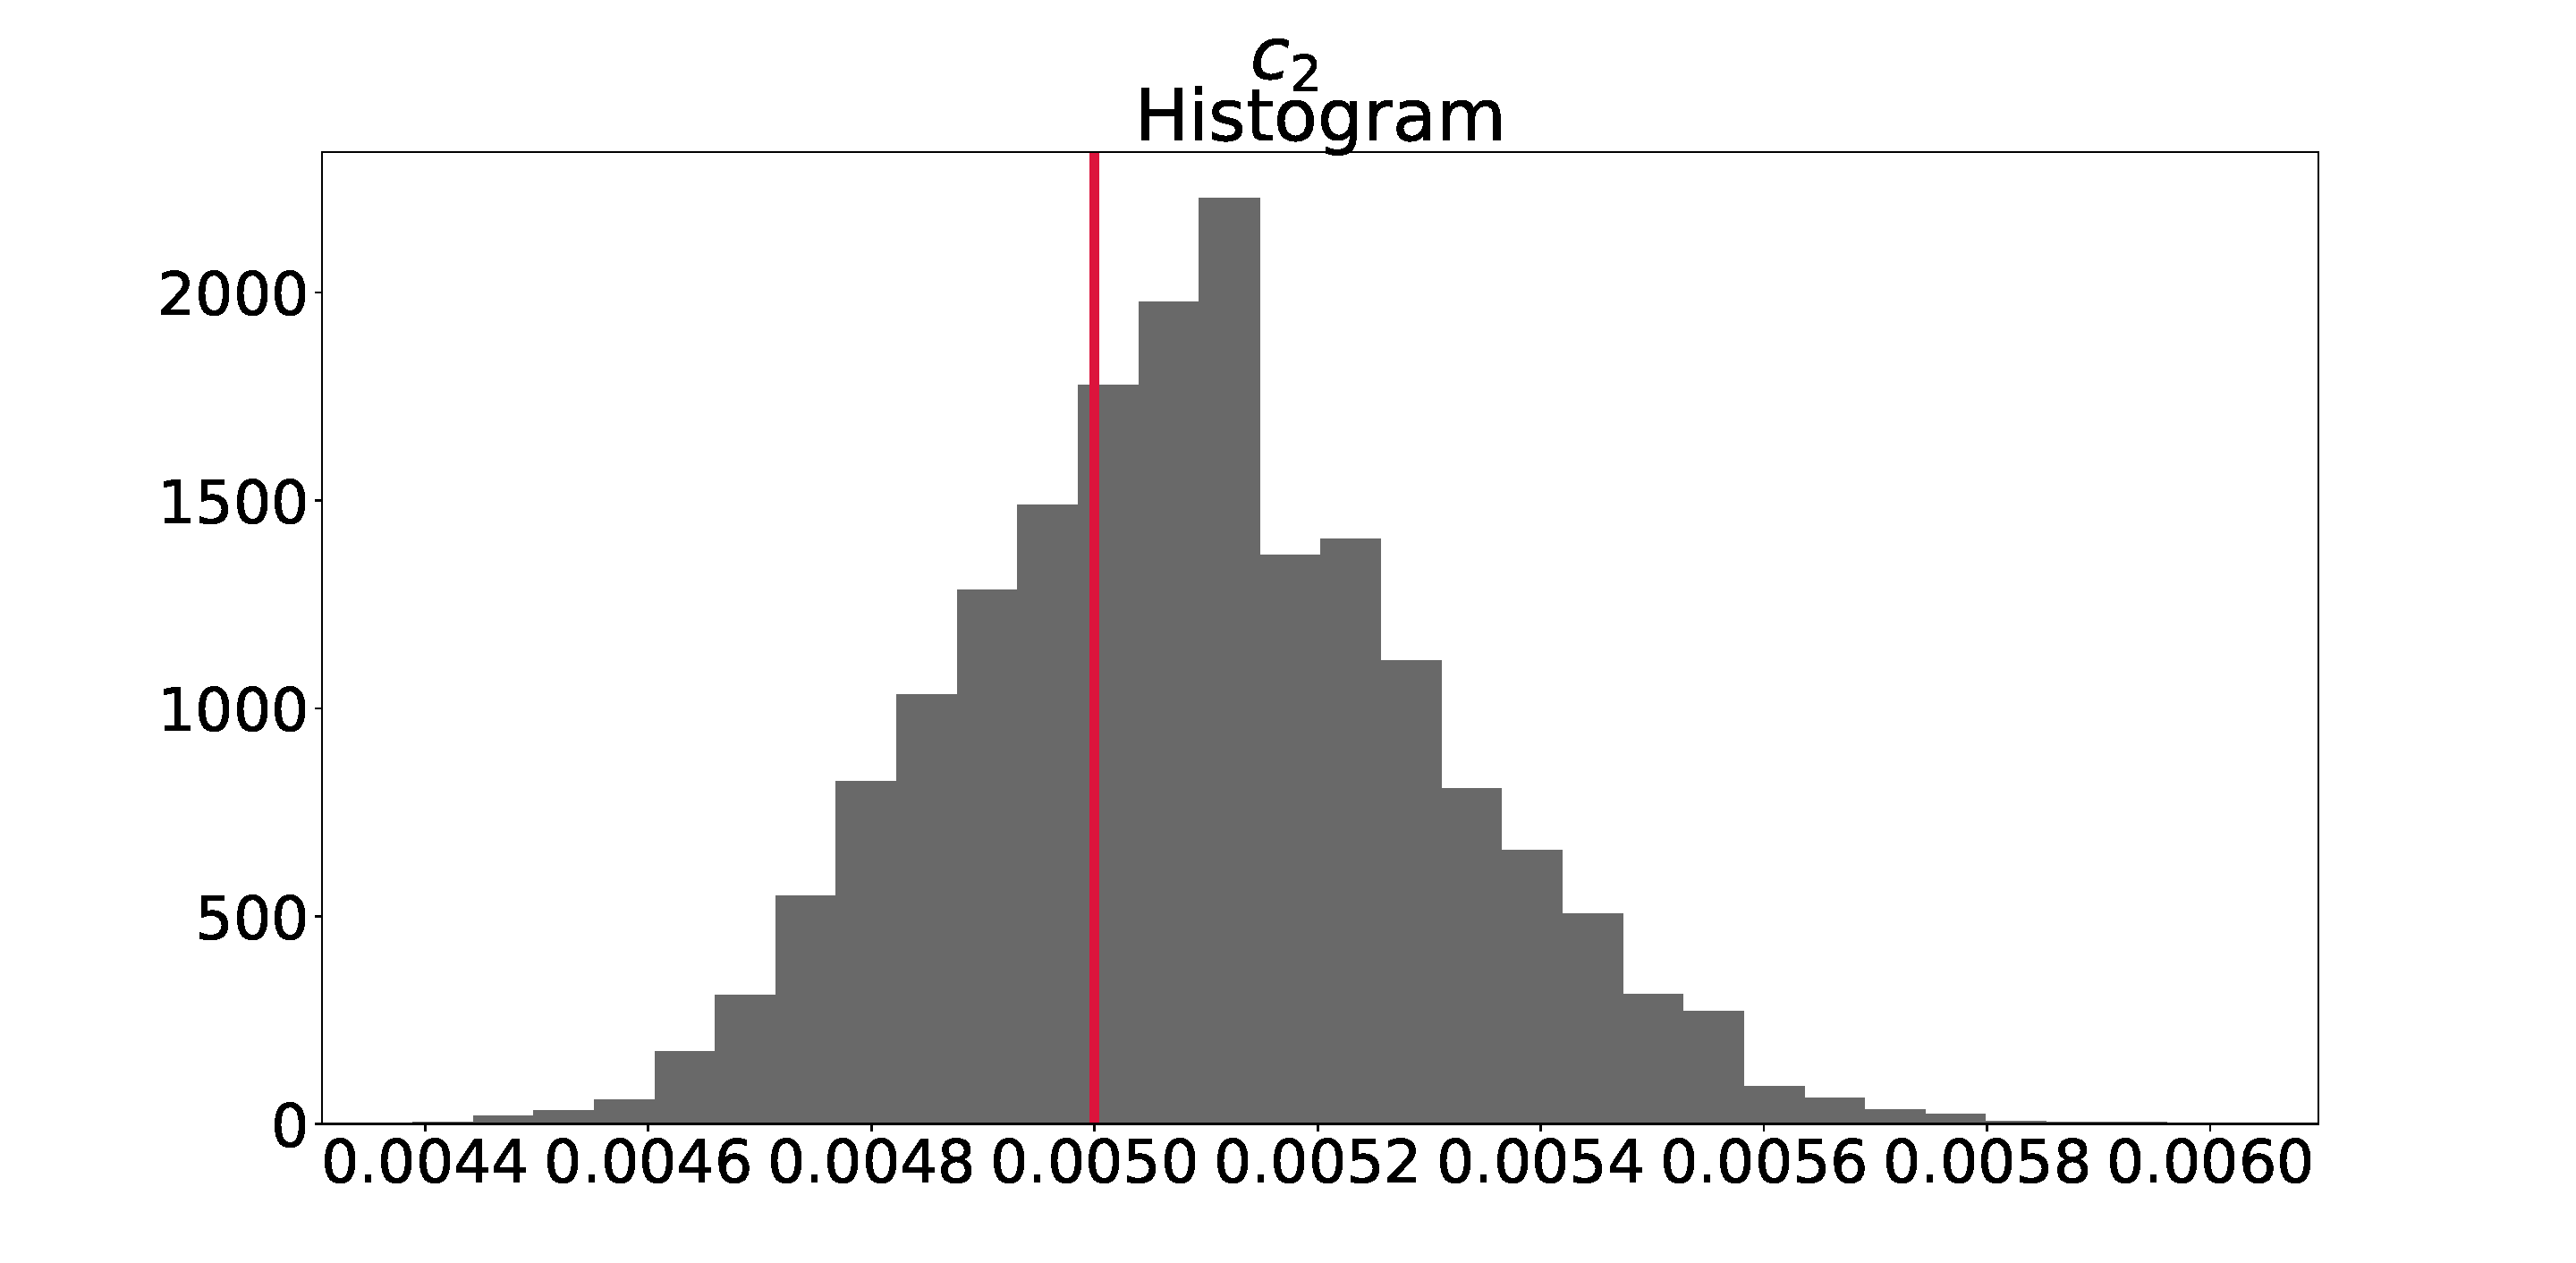
\includegraphics[width=\columnwidth]{images/lv_abc_c}
                \caption{Misspecified ABC.}
            \end{figure}
        \end{column}
    \end{columns}
    \end{frame}

    \begin{frame}
    \frametitle{Prokaryotic autoregulation model}
    \begin{columns}
        \begin{column}{0.4\textwidth}
            \begin{equation*}
            \begin{split}
            \mathcal{R}_1:\quad & \mathit{DNA} + P_2 \to \mathit{DNA} \cdot P_2 \\
            \mathcal{R}_2:\quad & \mathit{DNA} \cdot P_2 \to \mathit{DNA} + P_2 \\
            \mathcal{R}_3:\quad & \mathit{DNA} \to \mathit{DNA} + \mathit{RNA} \\
            \mathcal{R}_4:\quad & \mathit{RNA} \to \mathit{RNA} + P
            \end{split}
            \end{equation*}
        \end{column}
%
        \begin{column}{0.4\textwidth}
            \begin{equation*}
            \begin{split}
            \mathcal{R}_5:\quad & 2P \to P_2 \\
            \mathcal{R}_6:\quad & P_2 \to 2P \\
            \mathcal{R}_7:\quad & \mathit{RNA} \to \emptyset \\
            \mathcal{R}_8:\quad & P \to \emptyset
            \end{split}
            \end{equation*}
        \end{column}
    \end{columns}

    \begin{itemize}
        \item Unknown parameters $\btheta = \left(c_1, c_2, c_3, c_4, c_7, c_8\right)^\intercal$, Gaussian observation model.
        \item $\by_t = P_t + 2(P_2)_t$.
    \end{itemize}
    \end{frame}

    \begin{frame}
    \frametitle{Prokaryotic autoregulation model}
    \begin{columns}
        \begin{column}{0.45\textwidth}
            \begin{figure}
                \centering
                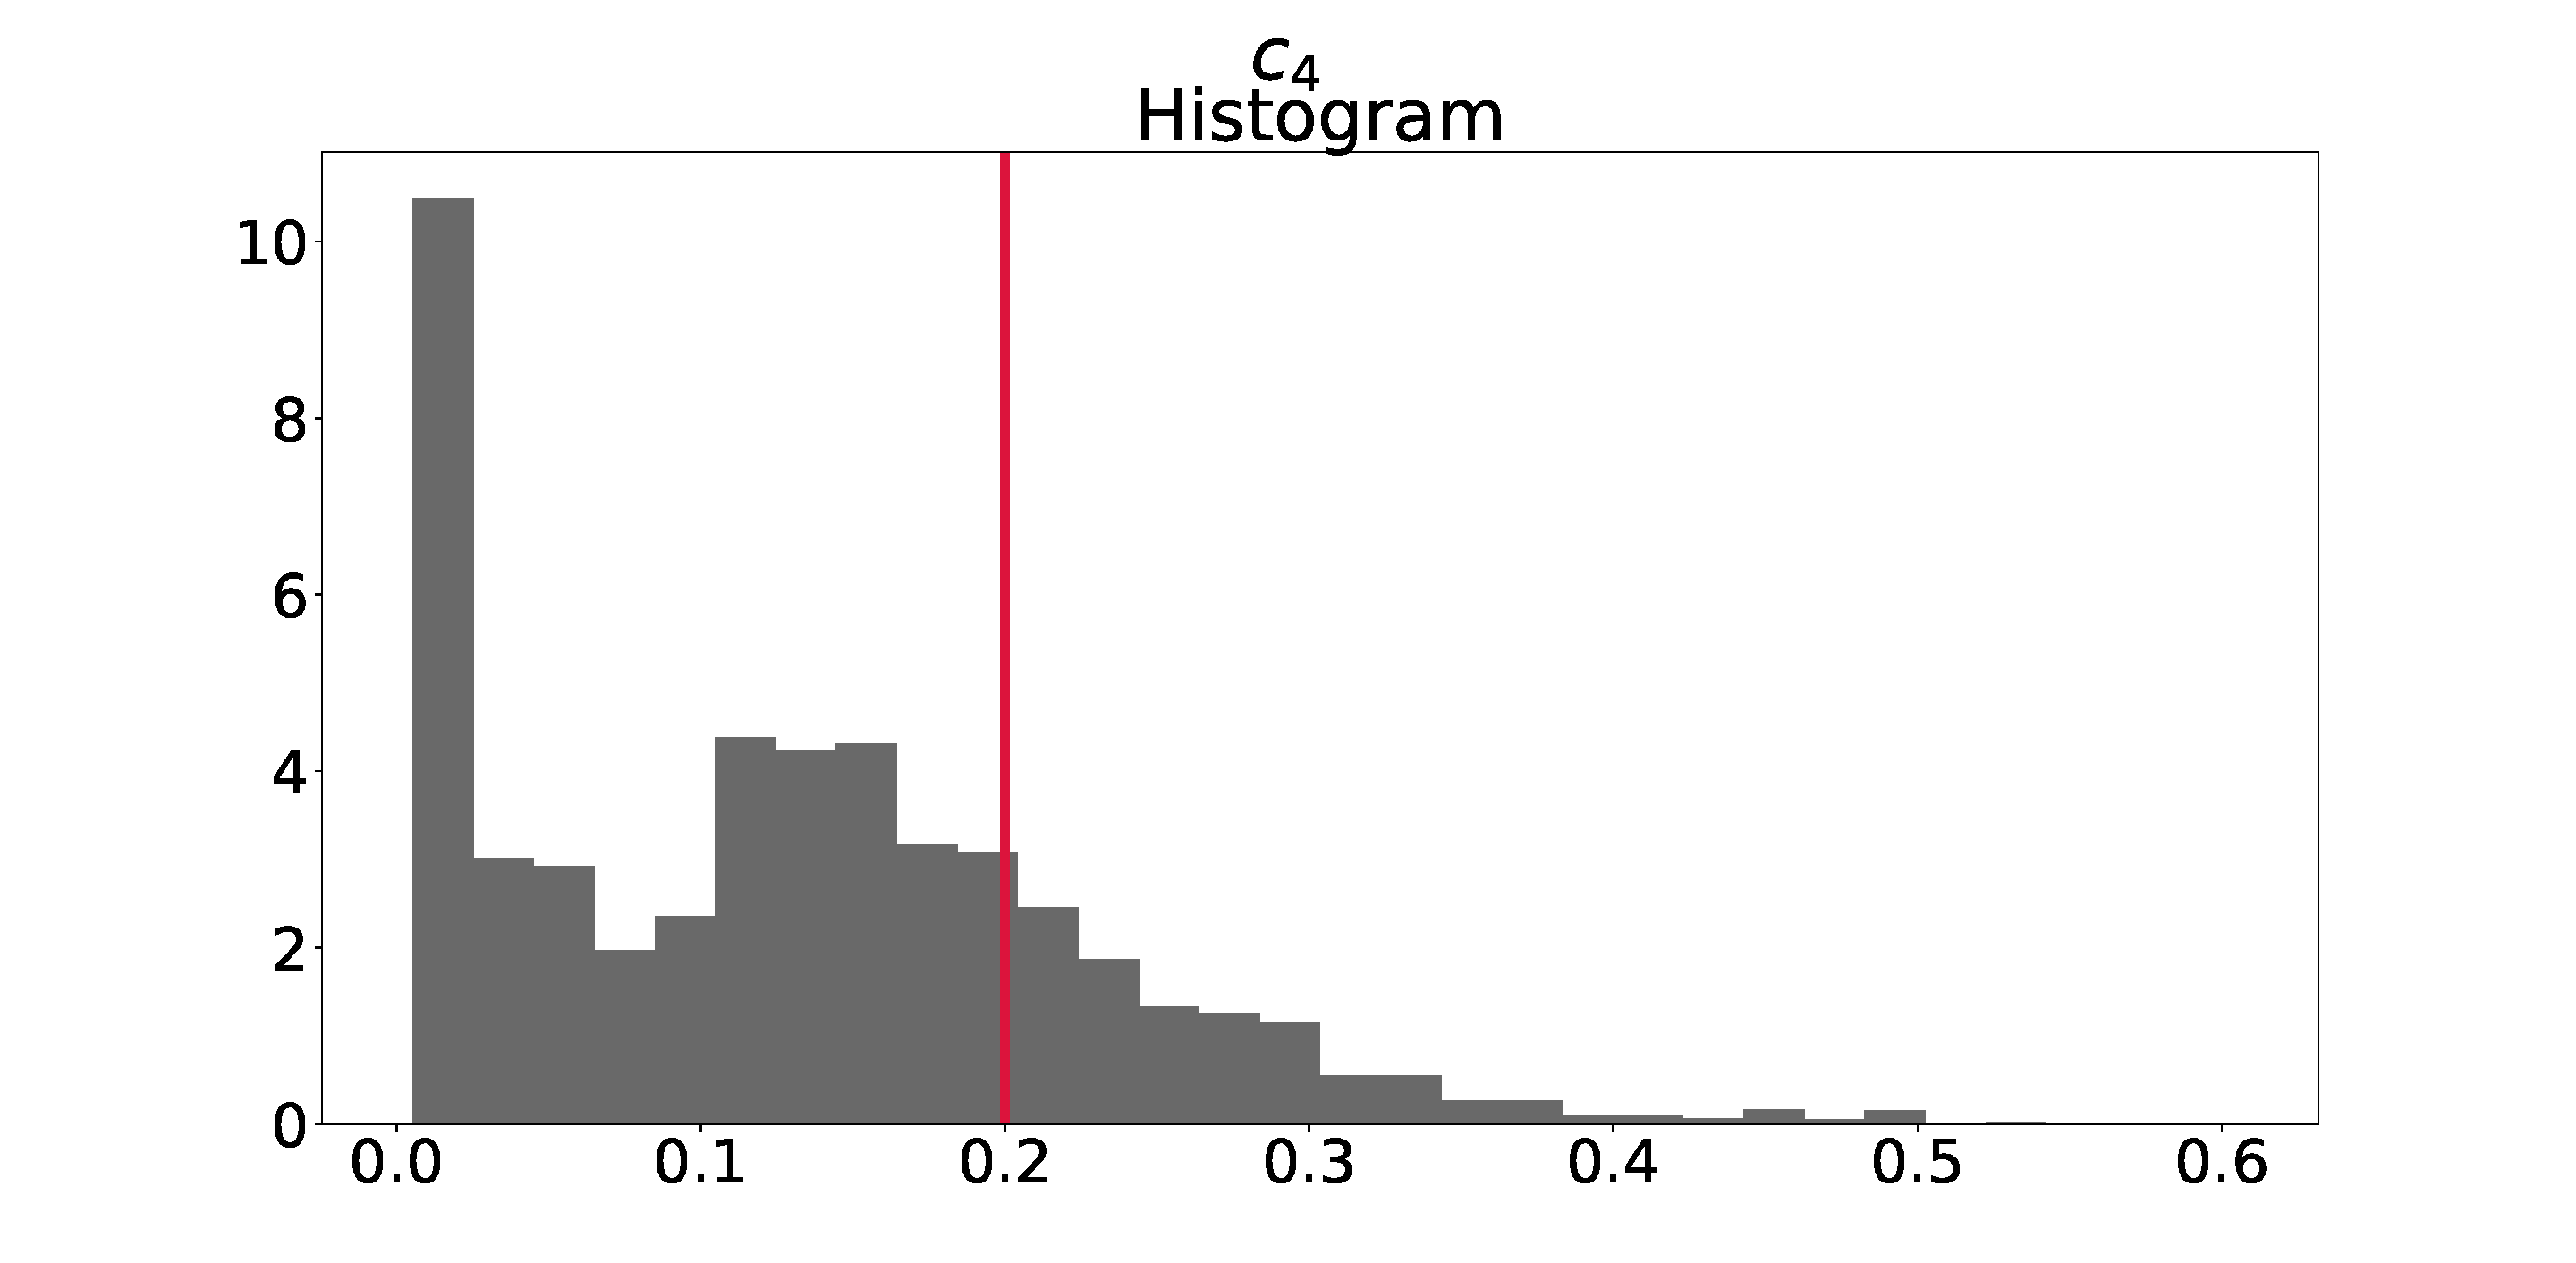
\includegraphics[width=\columnwidth]{images/ar_pf_g1}
                \caption{Well-specified PF.}
            \end{figure}
        \end{column}
        %
        \begin{column}{0.45\textwidth}
            \begin{figure}
                \centering
                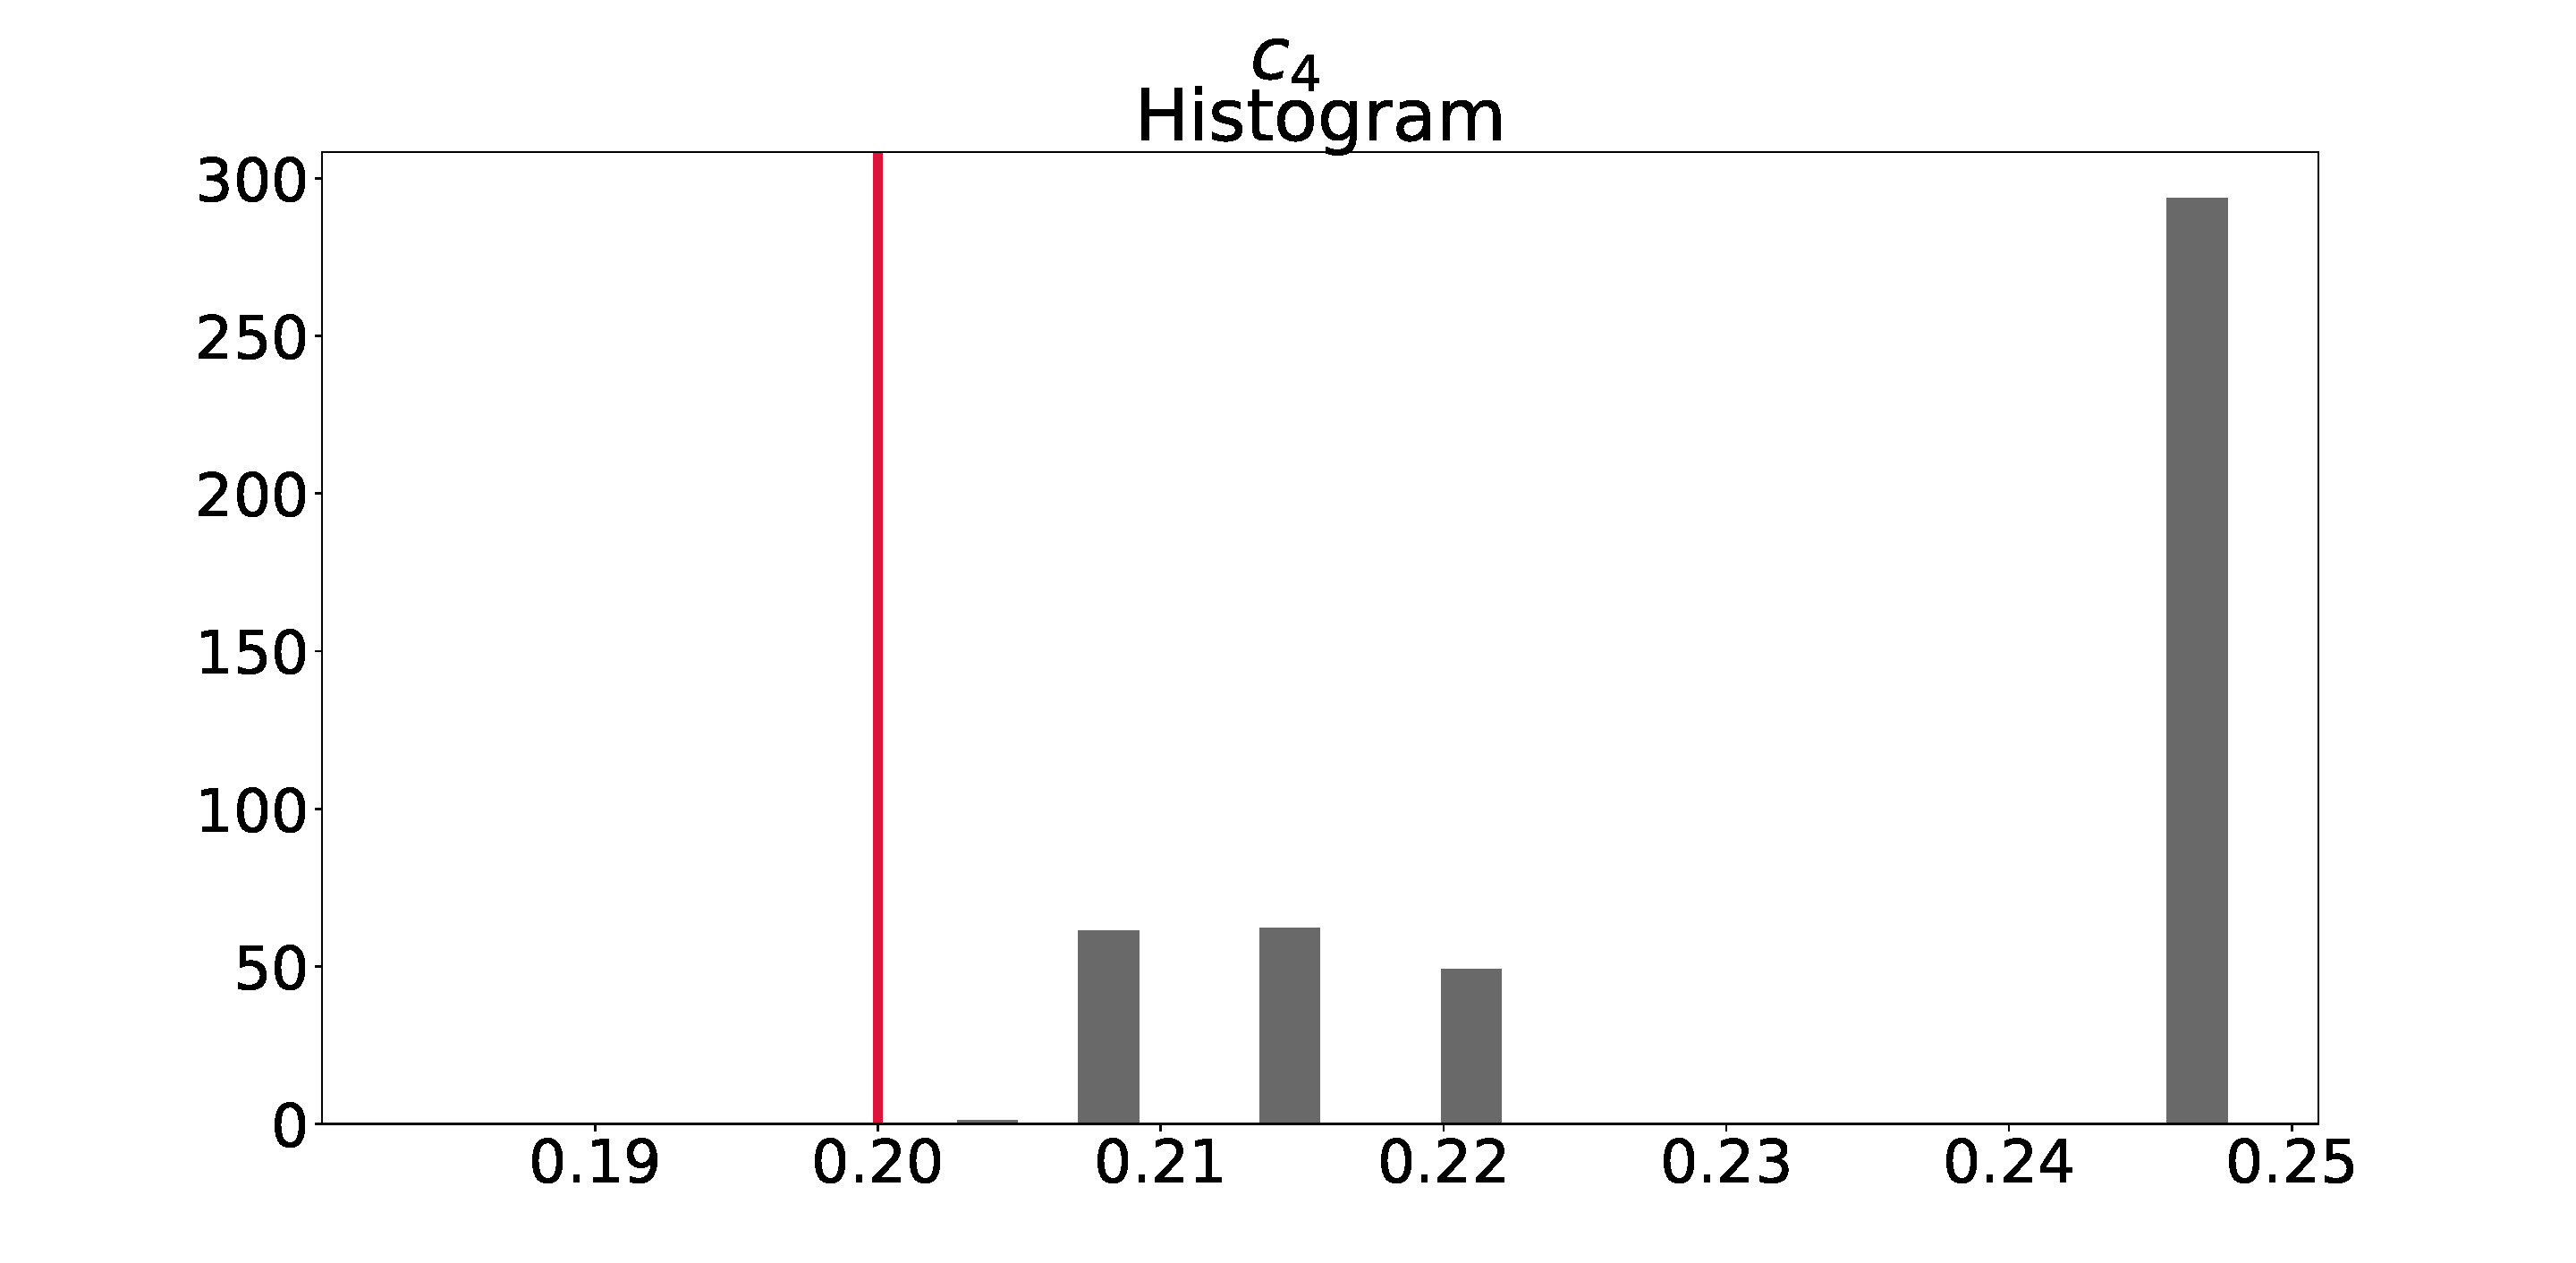
\includegraphics[width=\columnwidth]{images/ar_pf_c1}
                \caption{Misspecified PF.}
            \end{figure}
        \end{column}
    \end{columns}
    
    \begin{columns}
        \begin{column}{0.45\textwidth}
            \begin{figure}
                \centering
                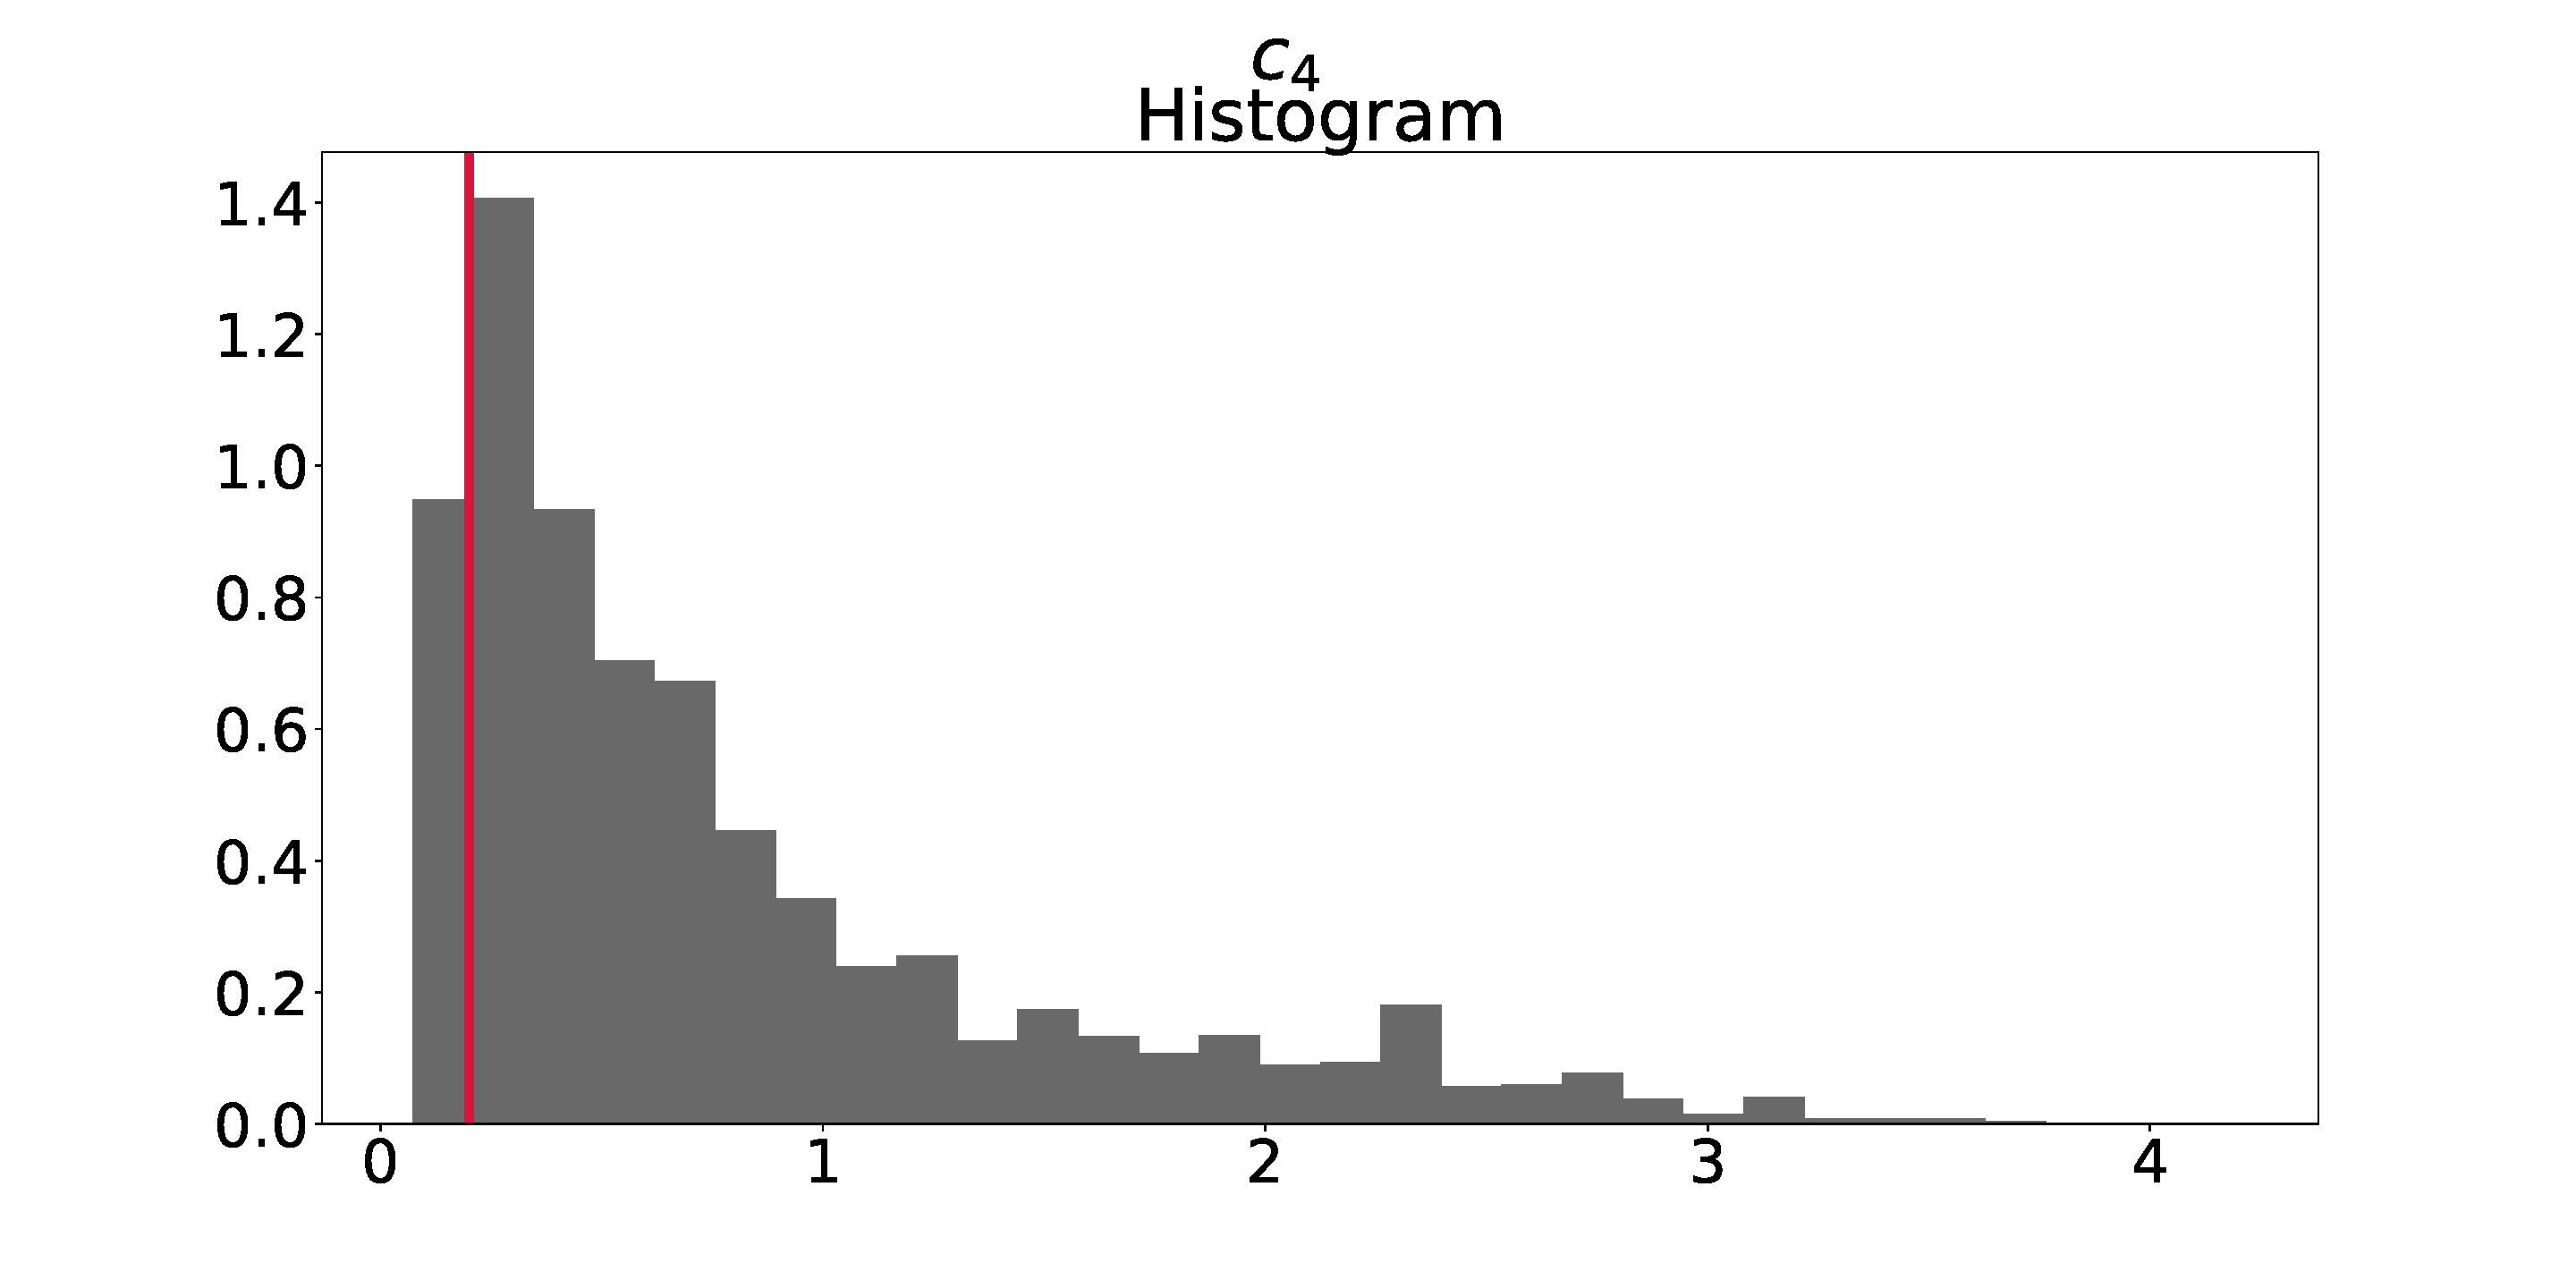
\includegraphics[width=\columnwidth]{images/ar_abc_g1}
                \caption{Well-specified ABC.}
            \end{figure}
        \end{column}
        %
        \begin{column}{0.45\textwidth}
            \begin{figure}
                \centering
                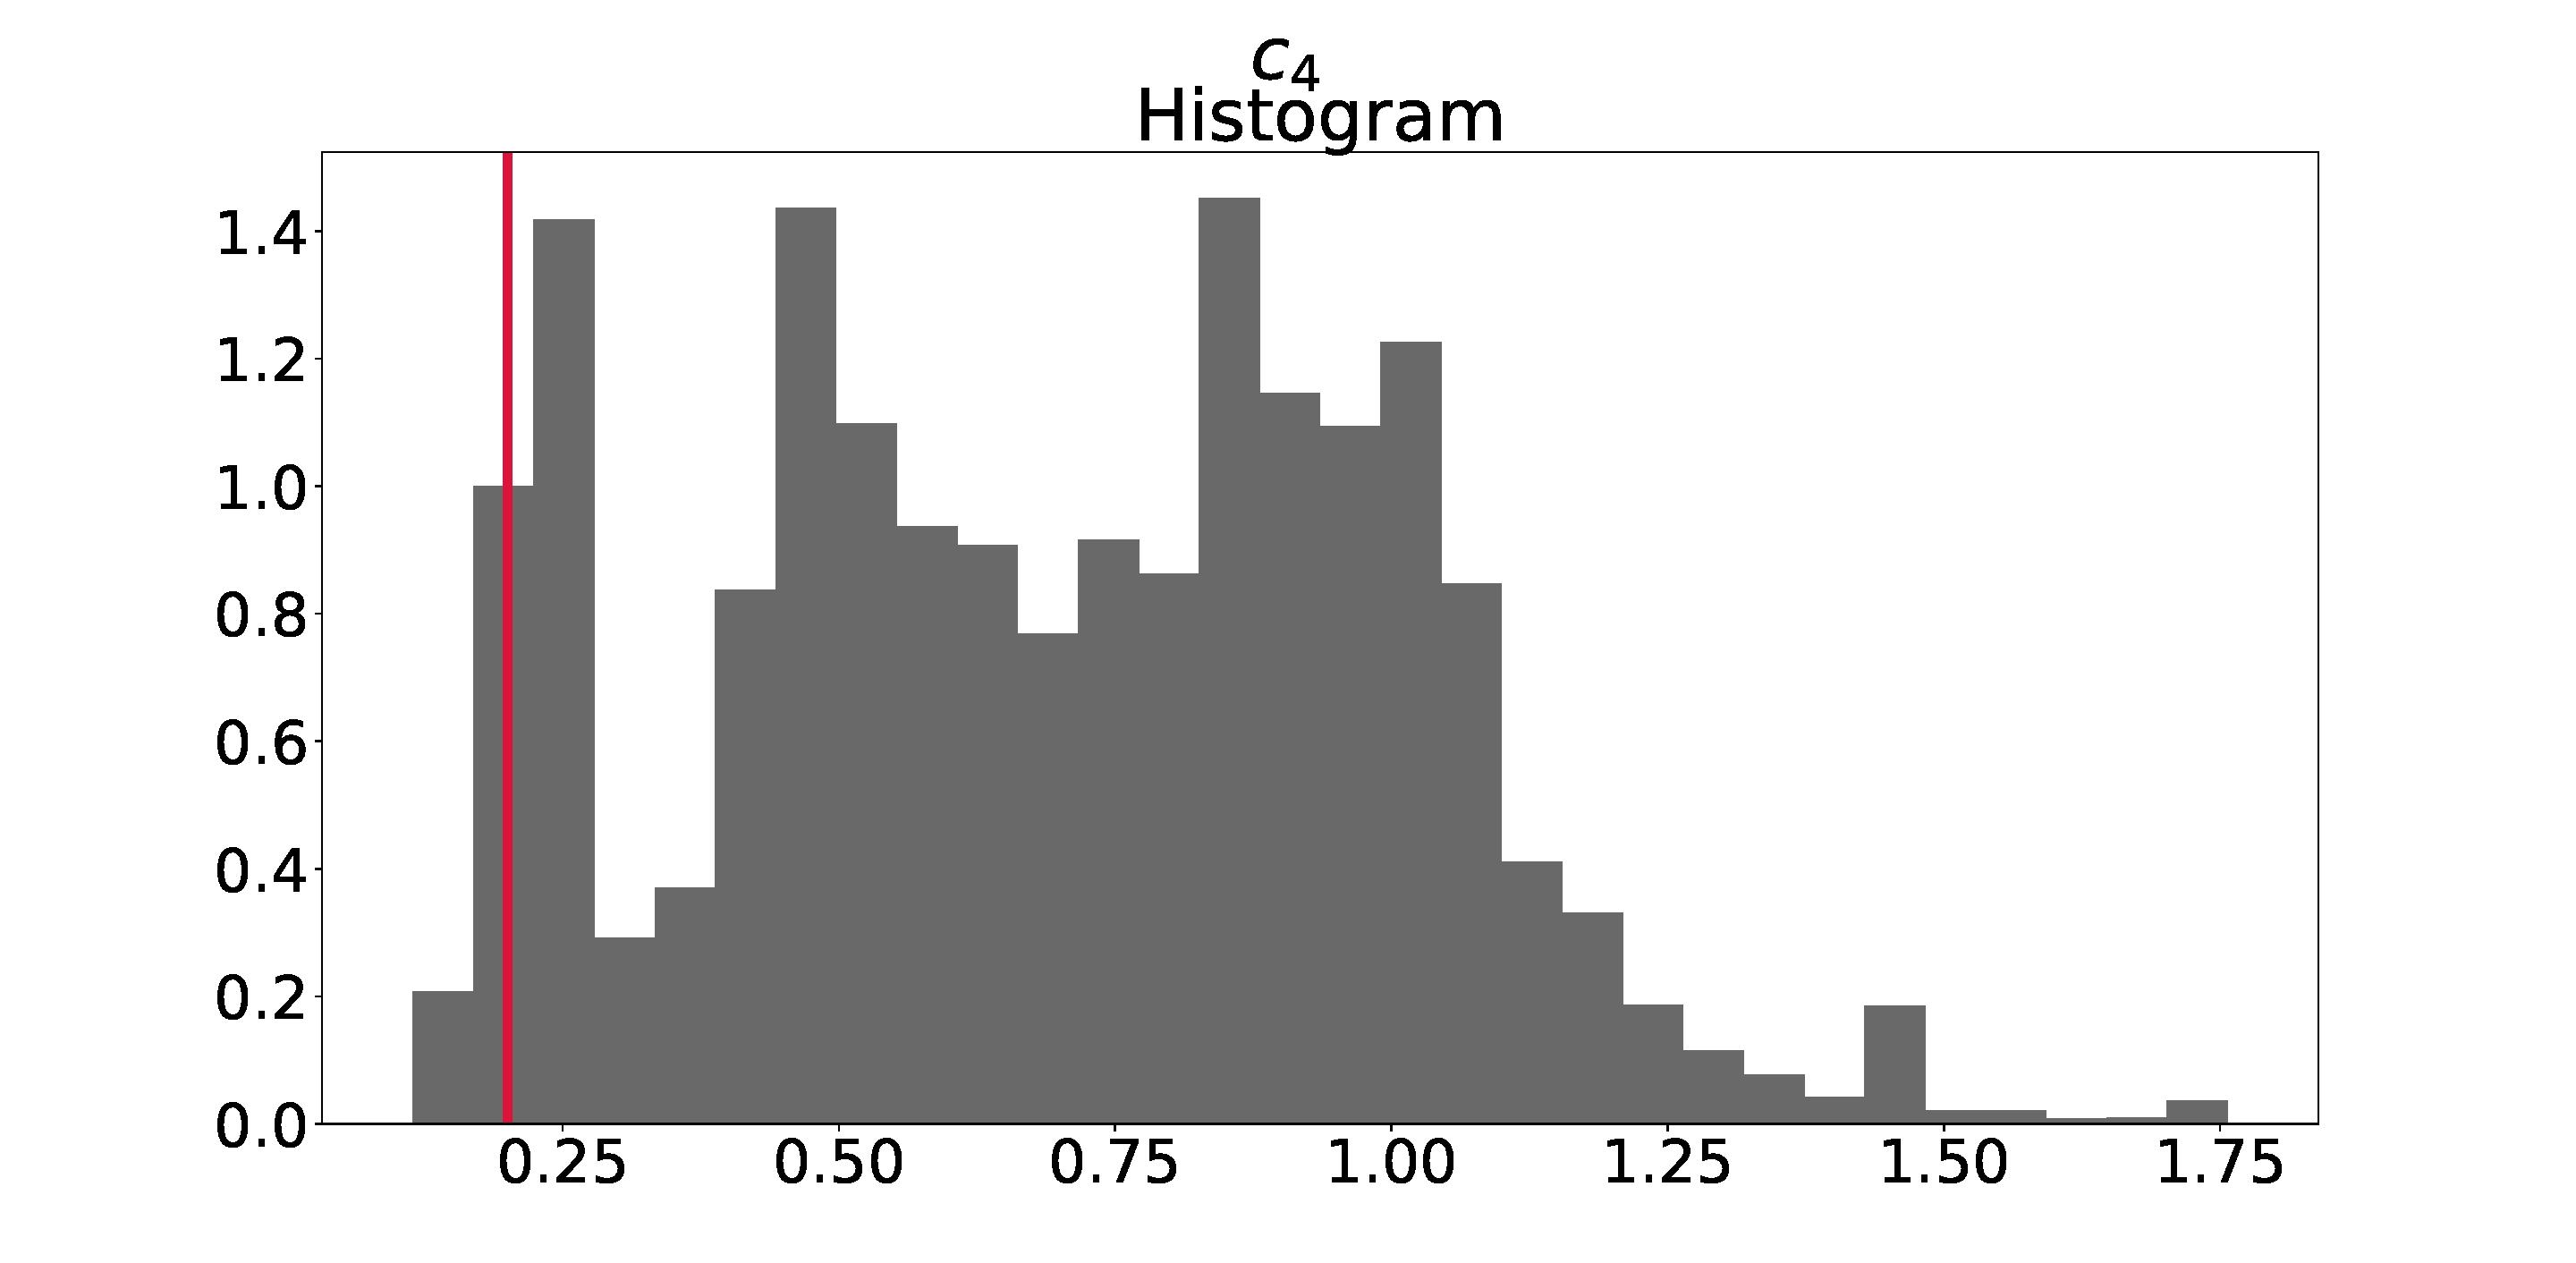
\includegraphics[width=\columnwidth]{images/ar_abc_c1}
                \caption{Misspecified ABC.}
            \end{figure}
        \end{column}
    \end{columns}
    \end{frame}

    \begin{frame}
    \frametitle{Prokaryotic autoregulation model}
    \begin{columns}
        \begin{column}{0.45\textwidth}
            \begin{figure}
                \centering
                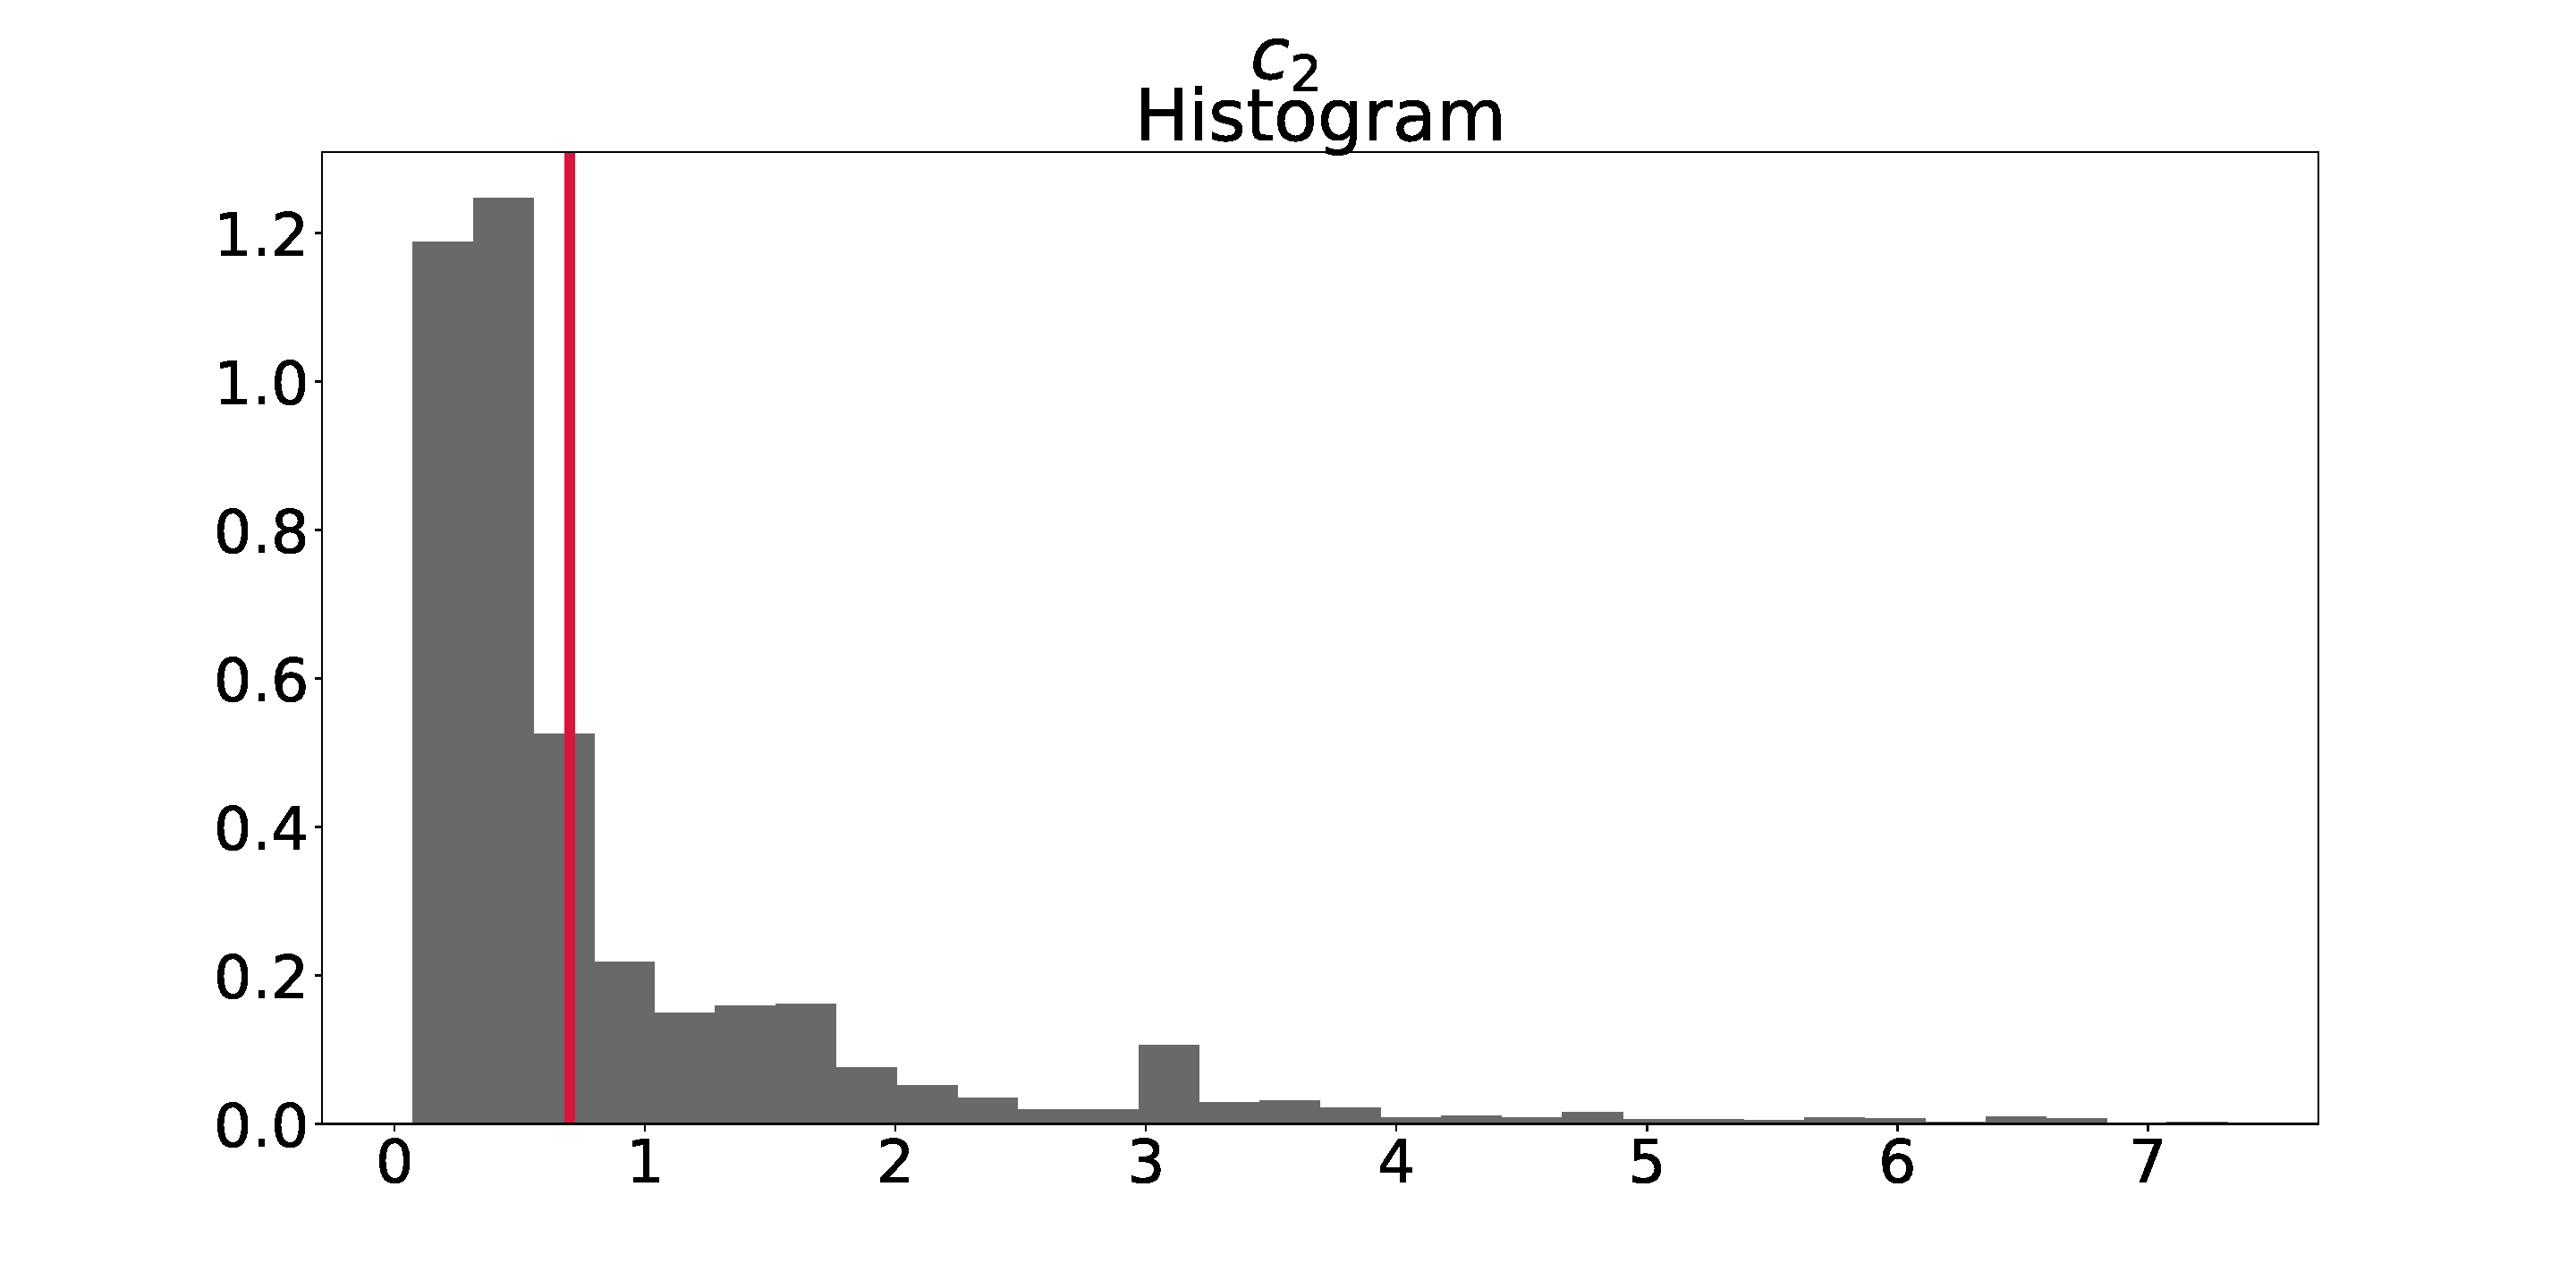
\includegraphics[width=\columnwidth]{images/ar_pf_g2}
                \caption{Well-specified PF.}
            \end{figure}
        \end{column}
        %
        \begin{column}{0.45\textwidth}
            \begin{figure}
                \centering
                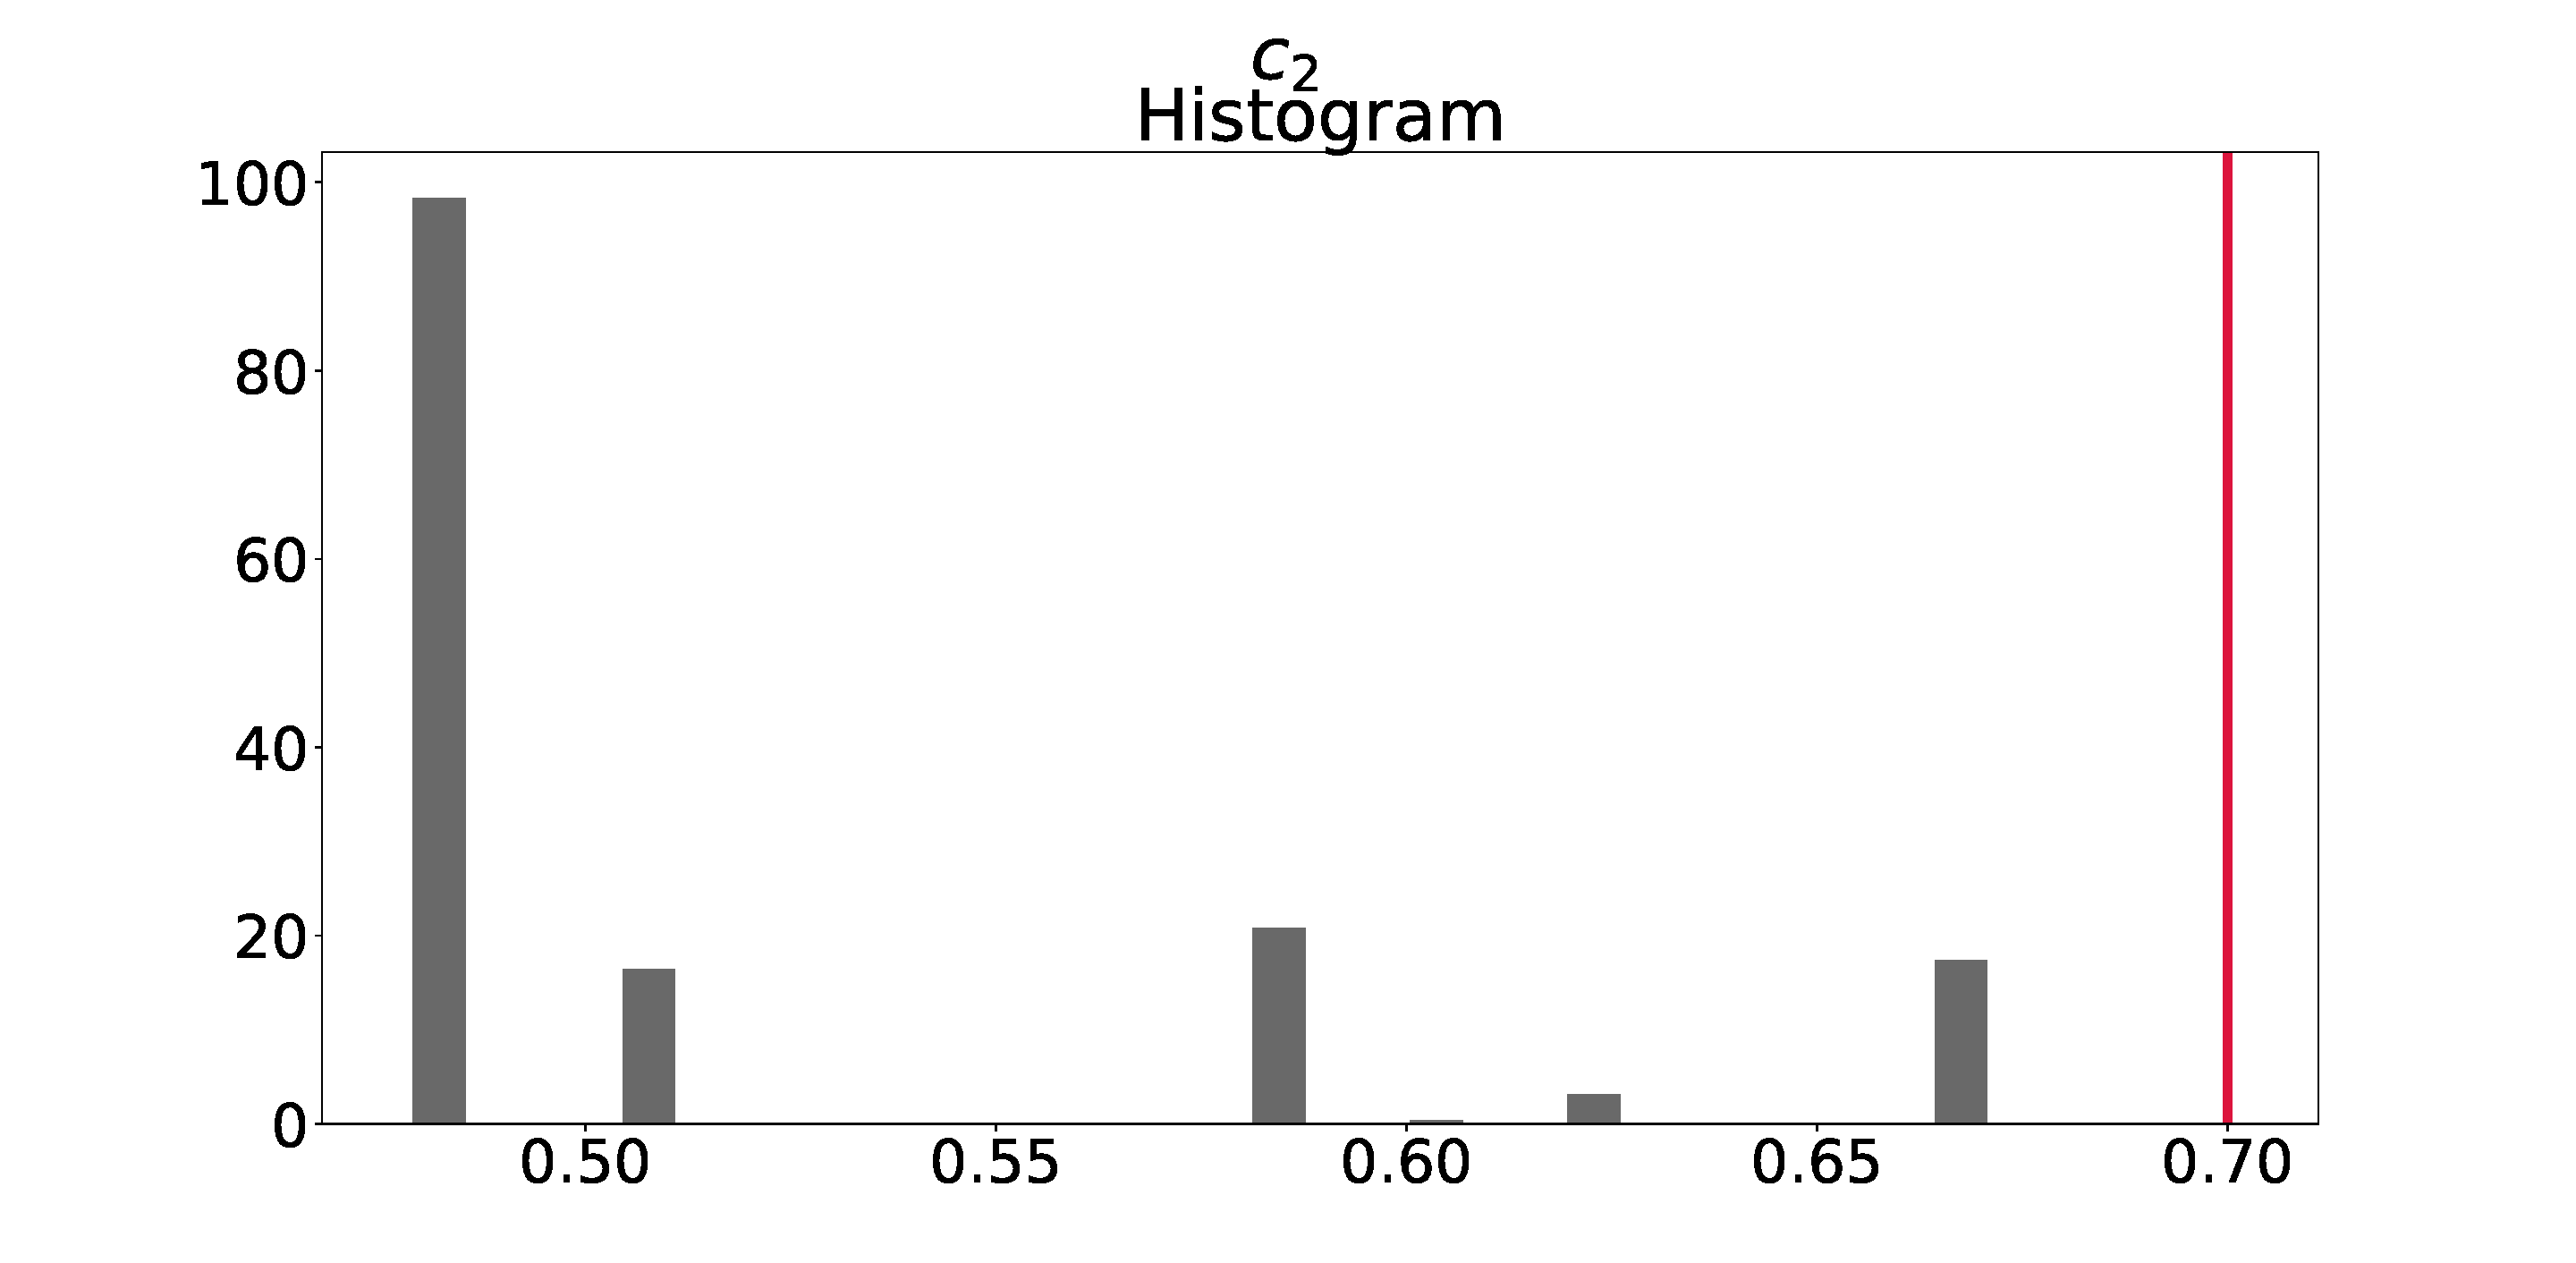
\includegraphics[width=\columnwidth]{images/ar_pf_c2}
                \caption{Misspecified PF.}
            \end{figure}
        \end{column}
    \end{columns}
    
    \begin{columns}
        \begin{column}{0.45\textwidth}
            \begin{figure}
                \centering
                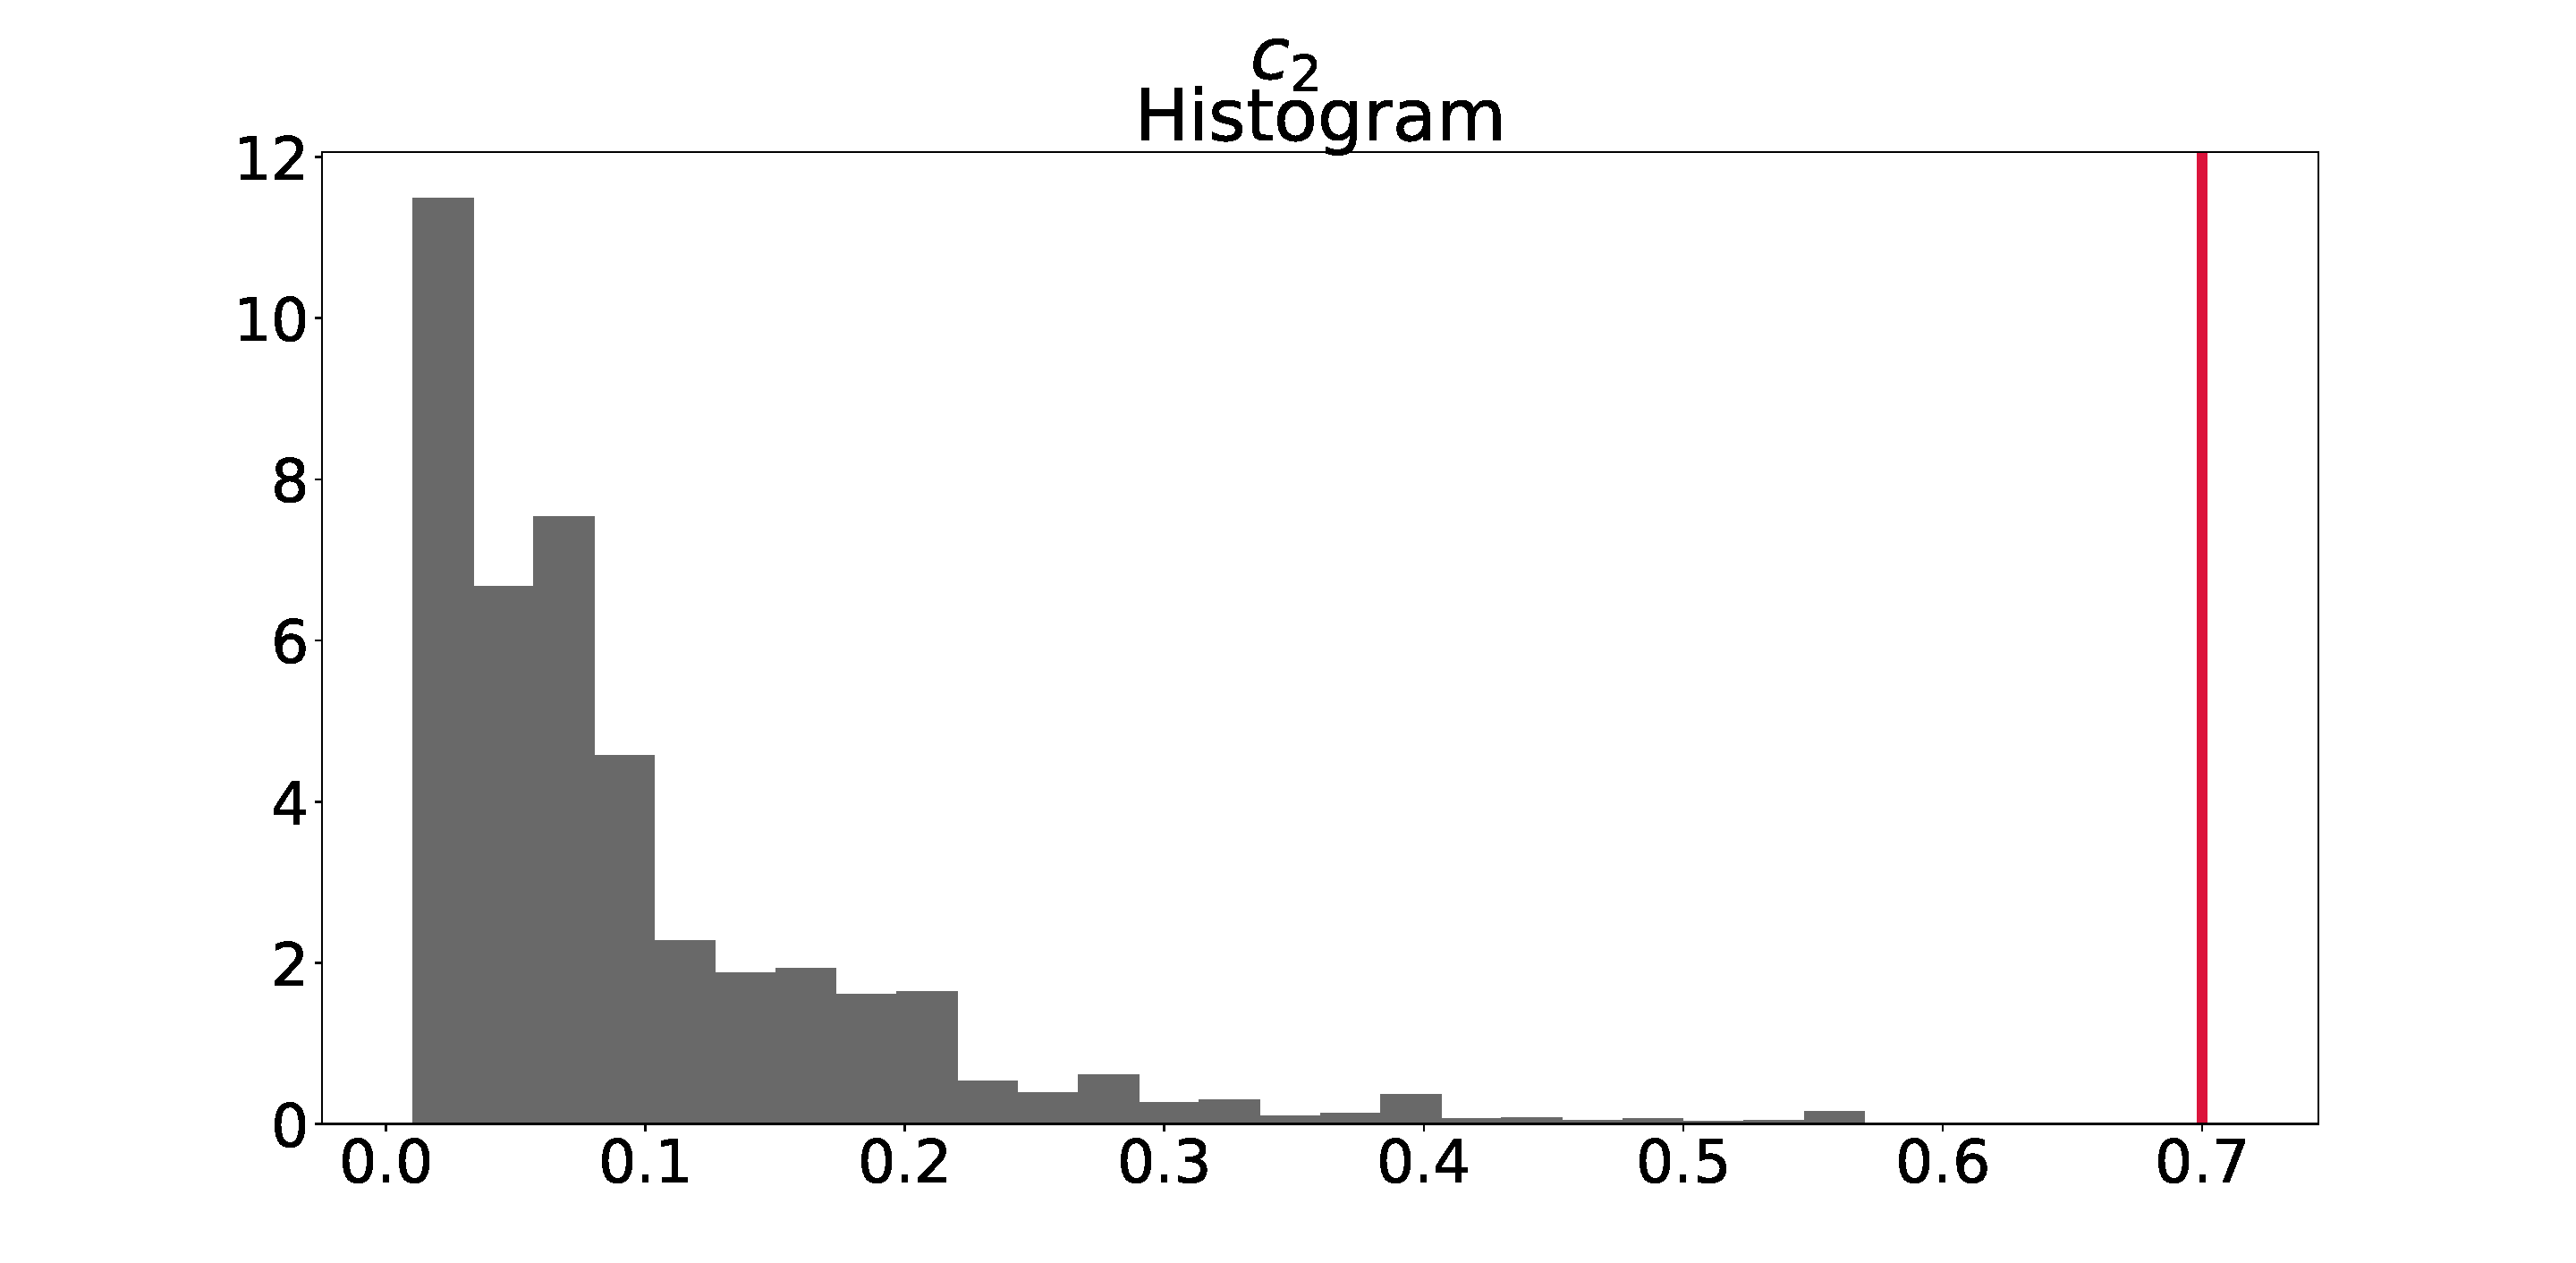
\includegraphics[width=\columnwidth]{images/ar_abc_g2}
                \caption{Well-specified ABC.}
            \end{figure}
        \end{column}
        %
        \begin{column}{0.45\textwidth}
            \begin{figure}
                \centering
                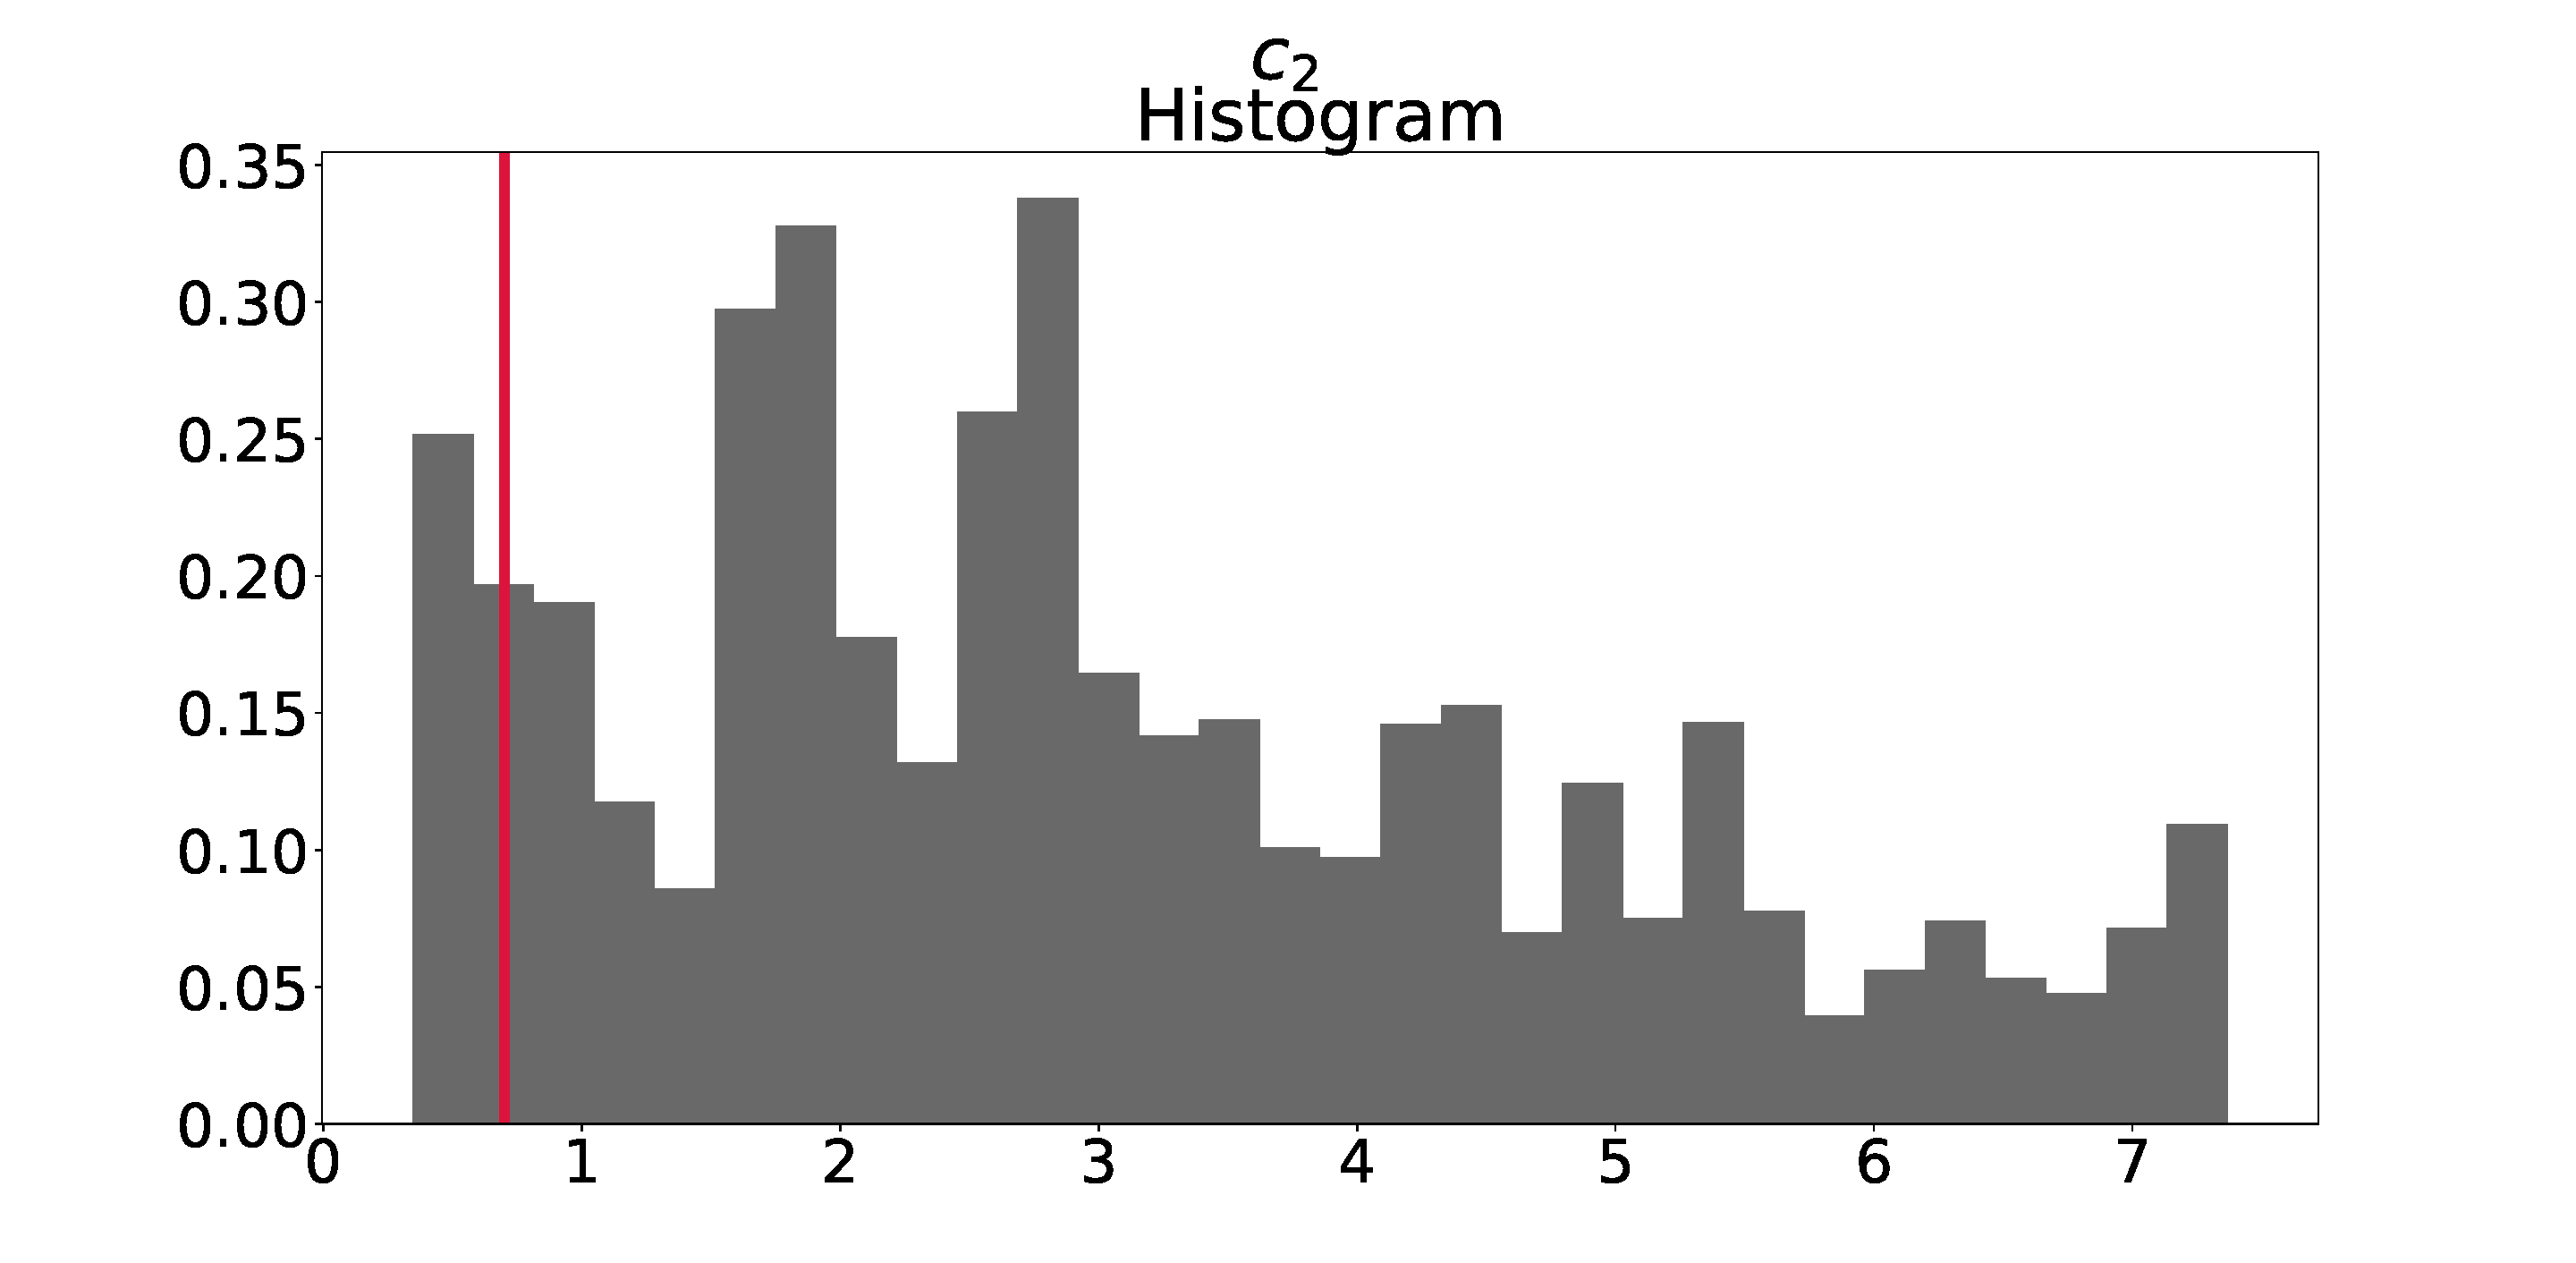
\includegraphics[width=\columnwidth]{images/ar_abc_c2}
                \caption{Misspecified ABC.}
            \end{figure}
        \end{column}
    \end{columns}
    \end{frame}

    \begin{frame}
    \frametitle{Summary}
    \begin{itemize}
        \item Static parameters complicate inference.
        \item Intractable likelihood can be approximated through the particle filter, assuming a known observation density $\obs_t(\by_t \mid \bx_t, \btheta)$.
        \item When only a deterministic observation process is available, ABC methods can be used instead.
        \item Robust to outliers and model misspecification.
        \item Flexibility in kernel choice.
    \end{itemize}
    \end{frame}

    \begin{frame}[noframenumbering]
    \frametitle{Gillespie algorithm}
    All operations for $i = 1, \ldots, v$, the number of reactions.
    \setbeamertemplate{enumerate items}[default]
    \begin{enumerate}
        \item Set  $t = 0$, initialize $\bx_t$.
        \item While $t \leq T$:
        \setbeamertemplate{enumerate items}[default]
        \begin{enumerate}
            \item Calculate $\displaystyle h_i(\bx_t, c_i) = c_i \prod_{j=1}^u \begin{pmatrix}
            x_{j,t} \\
            p_{ij}
            \end{pmatrix}$.
            \item Sample $\dx{t} \sim \mathcal{E}\mathit{xp}(\sum_{i=1}^v h_i(\bx_t, c_i))$.
            \item Sample $i$ with probability $\propto h_i(\bx_t, c_i)$.
            \item Set $\bx_{t+\dx{t}}$ by updating $\bx_t$ according to $\mathcal{R}_i$.
            \item $t = t + \dx{t}$.
        \end{enumerate}
        \item Output $\bx_t$, $t$.
    \end{enumerate}
    \end{frame}

    \begin{frame}[noframenumbering]
    \frametitle{ABC filter}
    All operations for $i = 1, \ldots, N$.
    \setbeamertemplate{enumerate items}[default]
    \begin{enumerate}
        \item Sample $\bx_0^{(i)} \sim \sprior(\bx_0 \mid \btheta)$, set $w_0^{(i)} = \frac{1}{N}$.
        \item For $t = 1, \ldots, T$:
        \setbeamertemplate{enumerate items}[default]
        \begin{enumerate}
            \item Sample $\bx_t^{(i)} \sim \trans_t(\bx_t \mid \bx_t^{(i)}, \btheta)$.
            \item Simulate $\bu_t^{(i)}$ from $\obs_t(\cdot \mid \bx_t^{(i)}, \btheta)$.
            \item Identify $\bu_t^{[\alpha]}$, the $\alpha$th closest pseudo-observation to $\by_t$.
            \item Set the kernel scale $\epsilon_t = \frac{\left| u_t^{[\alpha]} - y_t \right|}{F^{-1}(\frac{1+p}{2})}$.
            \item Set the weights $w_t^{(i)} \propto \kappa(\frac{\bu_t^{(i)} - \by_t}{\epsilon_t}) w_{t-1}^{(i)}.$
            \item Resample $\bx_t^{(i)}$ and reset $w_t^{(i)}$.
        \end{enumerate}
        \item Output $\left\{w_1^{(1)}, \ldots, w_1^{(N)}, \ldots, w_T^{(1)}, \ldots, w_T^{(N)}\right\}$.
    \end{enumerate}
    \end{frame}

    \begin{frame}[noframenumbering]
    \frametitle{ABC Metropolis-Hastings}
    \setbeamertemplate{enumerate items}[default]
    \begin{enumerate}
        \item Initialize $\btheta^{(0)}$, estimate $\widehat{p}(\by_{1:T} \mid \btheta^{(0)})$.
        \item For $m = 1, \ldots, M$:
        \setbeamertemplate{enumerate items}[default]
        \begin{enumerate}
            \item Propose $\btheta^\prime \sim q(\cdot \mid \btheta^{(m-1)})$.
            \item Estimate $\widehat{p}(\by_{1:T} \mid \btheta^\prime)$.
            \item Calculate the acceptance ratio
            \begin{equation*}
            \alpha = \min \left\{1, \frac{\widehat{p}(\by_{1:T} \mid \btheta^\prime) \pprior(\btheta^\prime)}{\widehat{p}(\by_{1:T} \mid \btheta^{(m-1)}) \pprior(\btheta^{(m-1)})} \frac{q(\btheta^{(m-1)} \mid \btheta^\prime)}{q(\btheta^\prime \mid \btheta^{(m-1)})} \right\}
            \end{equation*}
            \item With probability $\alpha$, set $\btheta^{(m)} = \btheta^\prime$. Otherwise, set $\btheta^{(m)} = \btheta^{(m-1)}$.
        \end{enumerate}
        \item Output $\left\{ \btheta^{(1)}, \ldots, \btheta^{(M)} \right\}$.
    \end{enumerate}
    \end{frame}
\end{document}